\section{Messungen und Ergebnisse}
\label{sec:results}

%% TODO: Dieses Kapitel ist bewusst noch ein Platzhalter für die eigentliche
%% QUARC-Portierung, Kraftsensor-Integration und Regelungsapplikation
%% (Anforderungen 1, 2 und 4 aus Abschnitt~\ref{sec:anforderungen}): diese
%% Arbeiten haben laut Projektstand noch nicht stattgefunden. Enthalten sind
%% bereits die abgeschlossene Baseline-Messung sowie die QUARC-Zykluszeit-
%% messung (beide zu Anforderung 3); die Ende-zu-Ende-Latenzmessung zum KRL-
%% Programm steht noch aus (siehe Abschnitt~\ref{sec:quarc_zykluszeit}).

\subsection{Baseline-Messung der MATLAB/KVP-Anbindung}
\label{sec:baseline}

Als Ausgangspunkt für Anforderung~3 (Erfassung und Analyse der
Ende-zu-Ende-Systemlatenzen) wurde die bestehende MATLAB/KVP-Anbindung
messtechnisch charakterisiert, bevor sie durch die QUARC-Struktur ersetzt
wird. Dazu wurde eine Kopie von Friesens Bahnskript
(\texttt{Bahnskript\_Messung.m}) um Timing-Instrumentierung ergänzt und eine
feste Quadratbahn (5 Wegpunkte, \ac{ptp}, $v=\SI{15}{\percent}$) fünfmal
identisch abgefahren (\texttt{m1}--\texttt{m5}, 24.08.2026). Auswertung und
Abbildungen erzeugt das MATLAB-Skript \texttt{auswertung\_baseline.m} (siehe
Anhang bzw.\ eingereichte Quelldateien); alle Zeitangaben stammen aus
\texttt{times.cycleTime} sowie den Teilzeiten \texttt{times.polltime},
\texttt{times.readtime}, \texttt{times.writetime} und \texttt{times.waittime}.

\subsubsection{Zykluszeit}

Tabelle~\ref{tab:baseline_zykluszeit} zeigt die Zykluszeit-Statistik pro Lauf
sowie gepoolt über alle 2218 gültigen Samples (jeweils ohne den ersten,
undefinierten Sample pro Lauf).

\begin{table}[H]
    \centering
    \caption{Zykluszeit-Statistik der MATLAB/KVP-Baseline in
    \si{\milli\second} (aus \texttt{cycleTime\_baseline\_stats.csv}).}
    \label{tab:baseline_zykluszeit}
    \begin{tabular}{lrrrrrrr}
        \toprule
        Lauf & $n$ & MW & Median & StdAbw & Min & Max & P95 \\
        \midrule
        Run 1 & 440 & 17.44 & 16.65 & 7.44 & 12.02 & 132.35 & 19.76 \\
        Run 2 & 447 & 17.14 & 16.65 & 5.00 & 12.14 & 68.90  & 19.29 \\
        Run 3 & 438 & 17.50 & 16.47 & 7.77 & 12.07 & 142.83 & 20.05 \\
        Run 4 & 446 & 17.17 & 16.56 & 5.09 & 13.14 & 69.85  & 19.73 \\
        Run 5 & 447 & 17.13 & 16.59 & 4.99 & 12.03 & 69.40  & 19.43 \\
        \midrule
        Gesamt (gepoolt) & 2218 & \textbf{17.27} & \textbf{16.58} & 6.18 & 12.02 & 142.83 & 19.62 \\
        \bottomrule
    \end{tabular}
\end{table}

Die Steuerung aktualisiert ihre \ac{krl}-Variablen nur alle
\SI{12}{\milli\second} (vgl.\ Abschnitt~\ref{sec:friesen}); das Messskript
wartet entsprechend mindestens diese Zeit pro Zyklus ab. Der gepoolte Median
liegt mit \SI{16.6}{\milli\second} rund \SI{4.5}{\milli\second} über dieser
Vorgabe. Da die gemessenen Teilzeiten (Abschnitt~\ref{sec:baseline_teilzeiten})
im Mittel nur ca.\ \SI{1.5}{\milli\second} betragen, liegt diese Differenz
außerhalb der eigentlichen \ac{tcpip}-Kommunikation und ist als
MATLAB-/Windows-Scheduling-Overhead einzuordnen.

\begin{figure}[H]
    \centering
    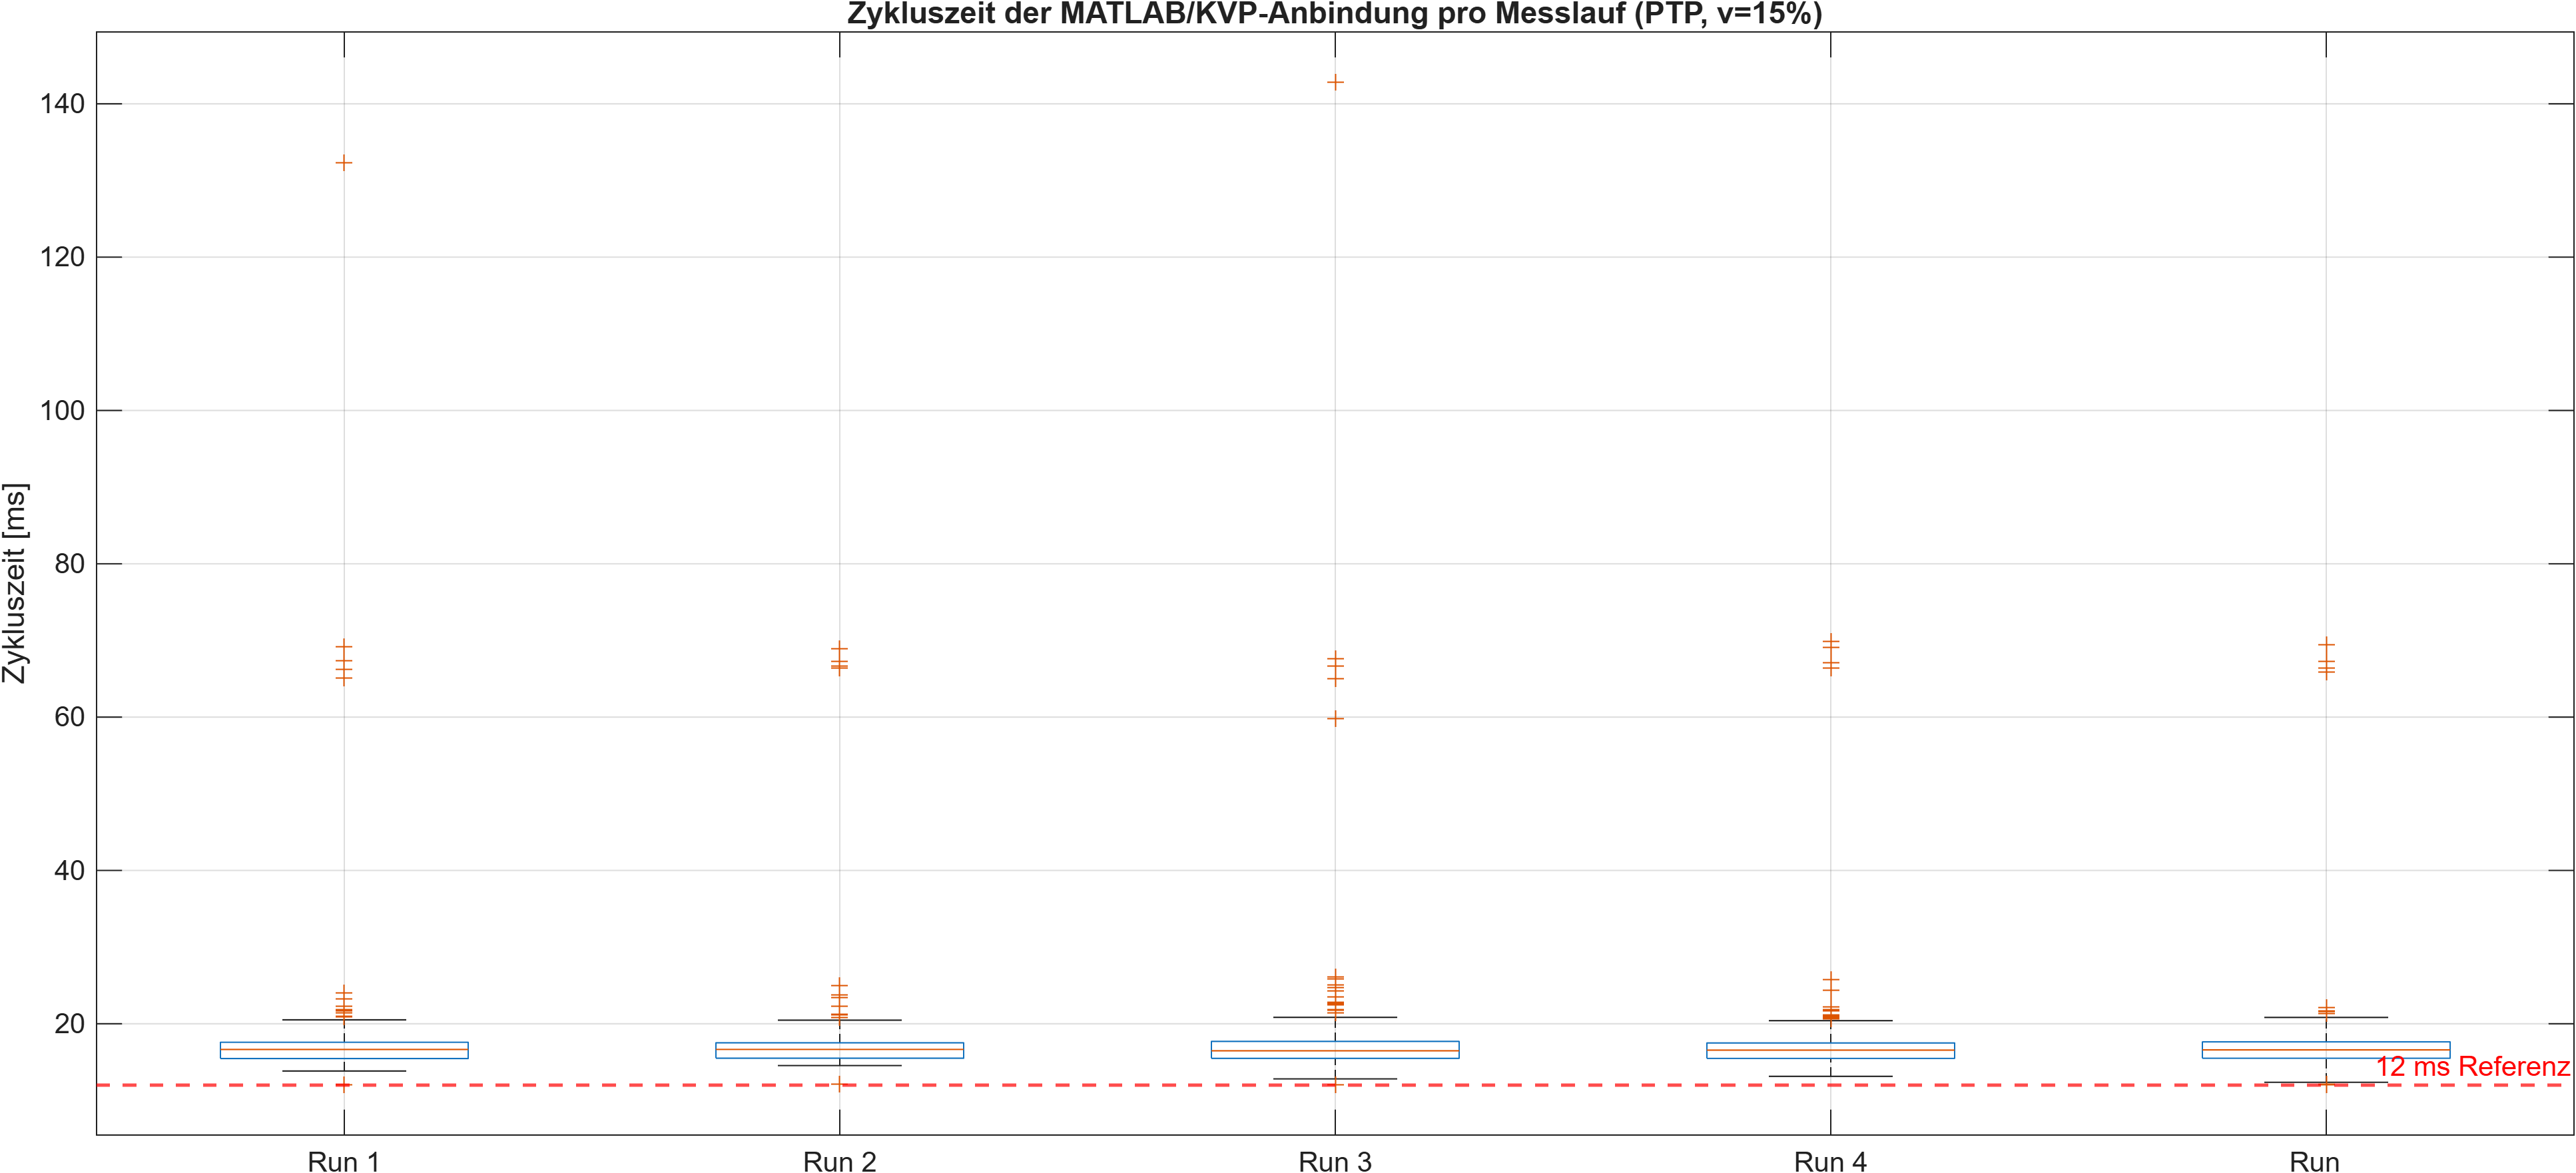
\includegraphics[width=0.75\linewidth]{images/zykluszeit_boxplot.png}
    \caption{Zykluszeit pro Messlauf (Boxplot), erzeugt mit
    \texttt{auswertung\_baseline.m}.}
    \label{fig:baseline_boxplot}
\end{figure}

\begin{figure}[H]
    \centering
    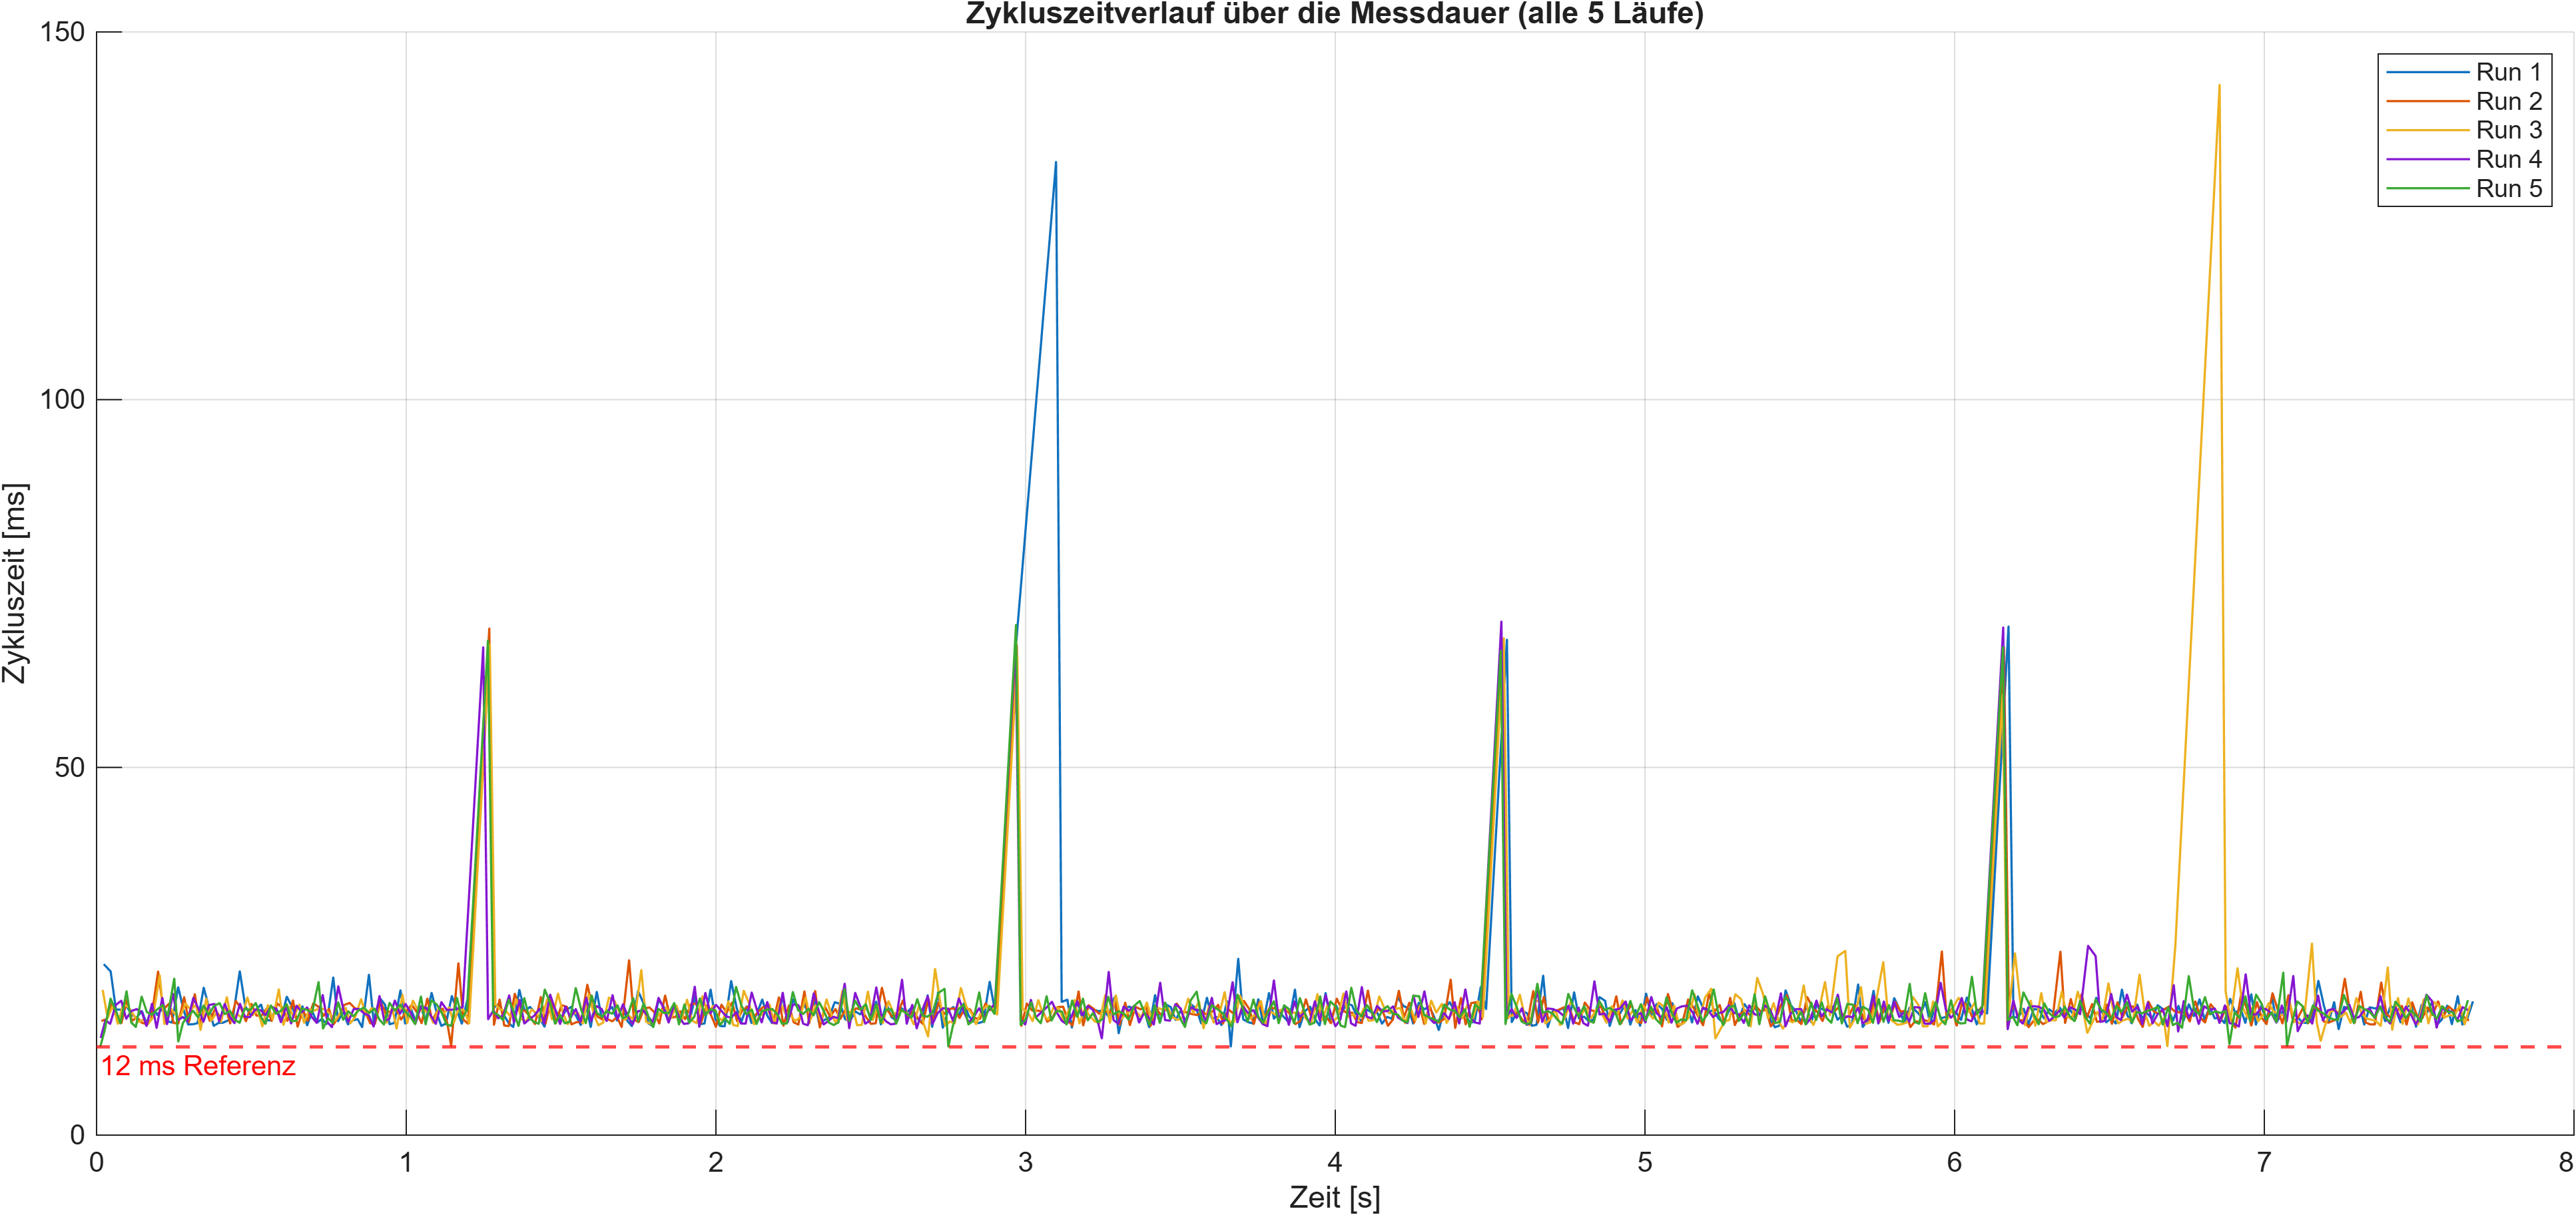
\includegraphics[width=0.9\linewidth]{images/zykluszeit_zeitverlauf.png}
    \caption{Zeitverlauf der Zykluszeit über alle 5 Läufe, mit
    \SI{12}{\milli\second}-Referenzlinie.}
    \label{fig:baseline_zeitverlauf}
\end{figure}

\subsubsection{Teilzeiten und Peak-Ursachen}
\label{sec:baseline_teilzeiten}

Tabelle~\ref{tab:baseline_teilzeiten} schlüsselt die Zykluszeit gepoolt über
alle 5 Läufe in ihre Teilzeiten auf.

\begin{table}[H]
    \centering
    \caption{Teilzeiten der MATLAB/KVP-Anbindung in \si{\milli\second},
    gepoolt über alle 5 Läufe.}
    \label{tab:baseline_teilzeiten}
    \begin{tabular}{lrrrrr}
        \toprule
        Größe & MW & Median & StdAbw & Min & Max \\
        \midrule
        polltime  & 1.46 & 0.98 & 4.23 & 0.56 & 142.75 \\
        readtime  & 0.79 & 0.38 & 4.19 & 0.09 & 141.87 \\
        writetime & 0.38 & 0.27 & 0.29 & 0.14 & 3.61 \\
        waittime  & 0.13 & 0.09 & 0.17 & 0.05 & 3.50 \\
        \bottomrule
    \end{tabular}
\end{table}

\begin{figure}[H]
    \centering
    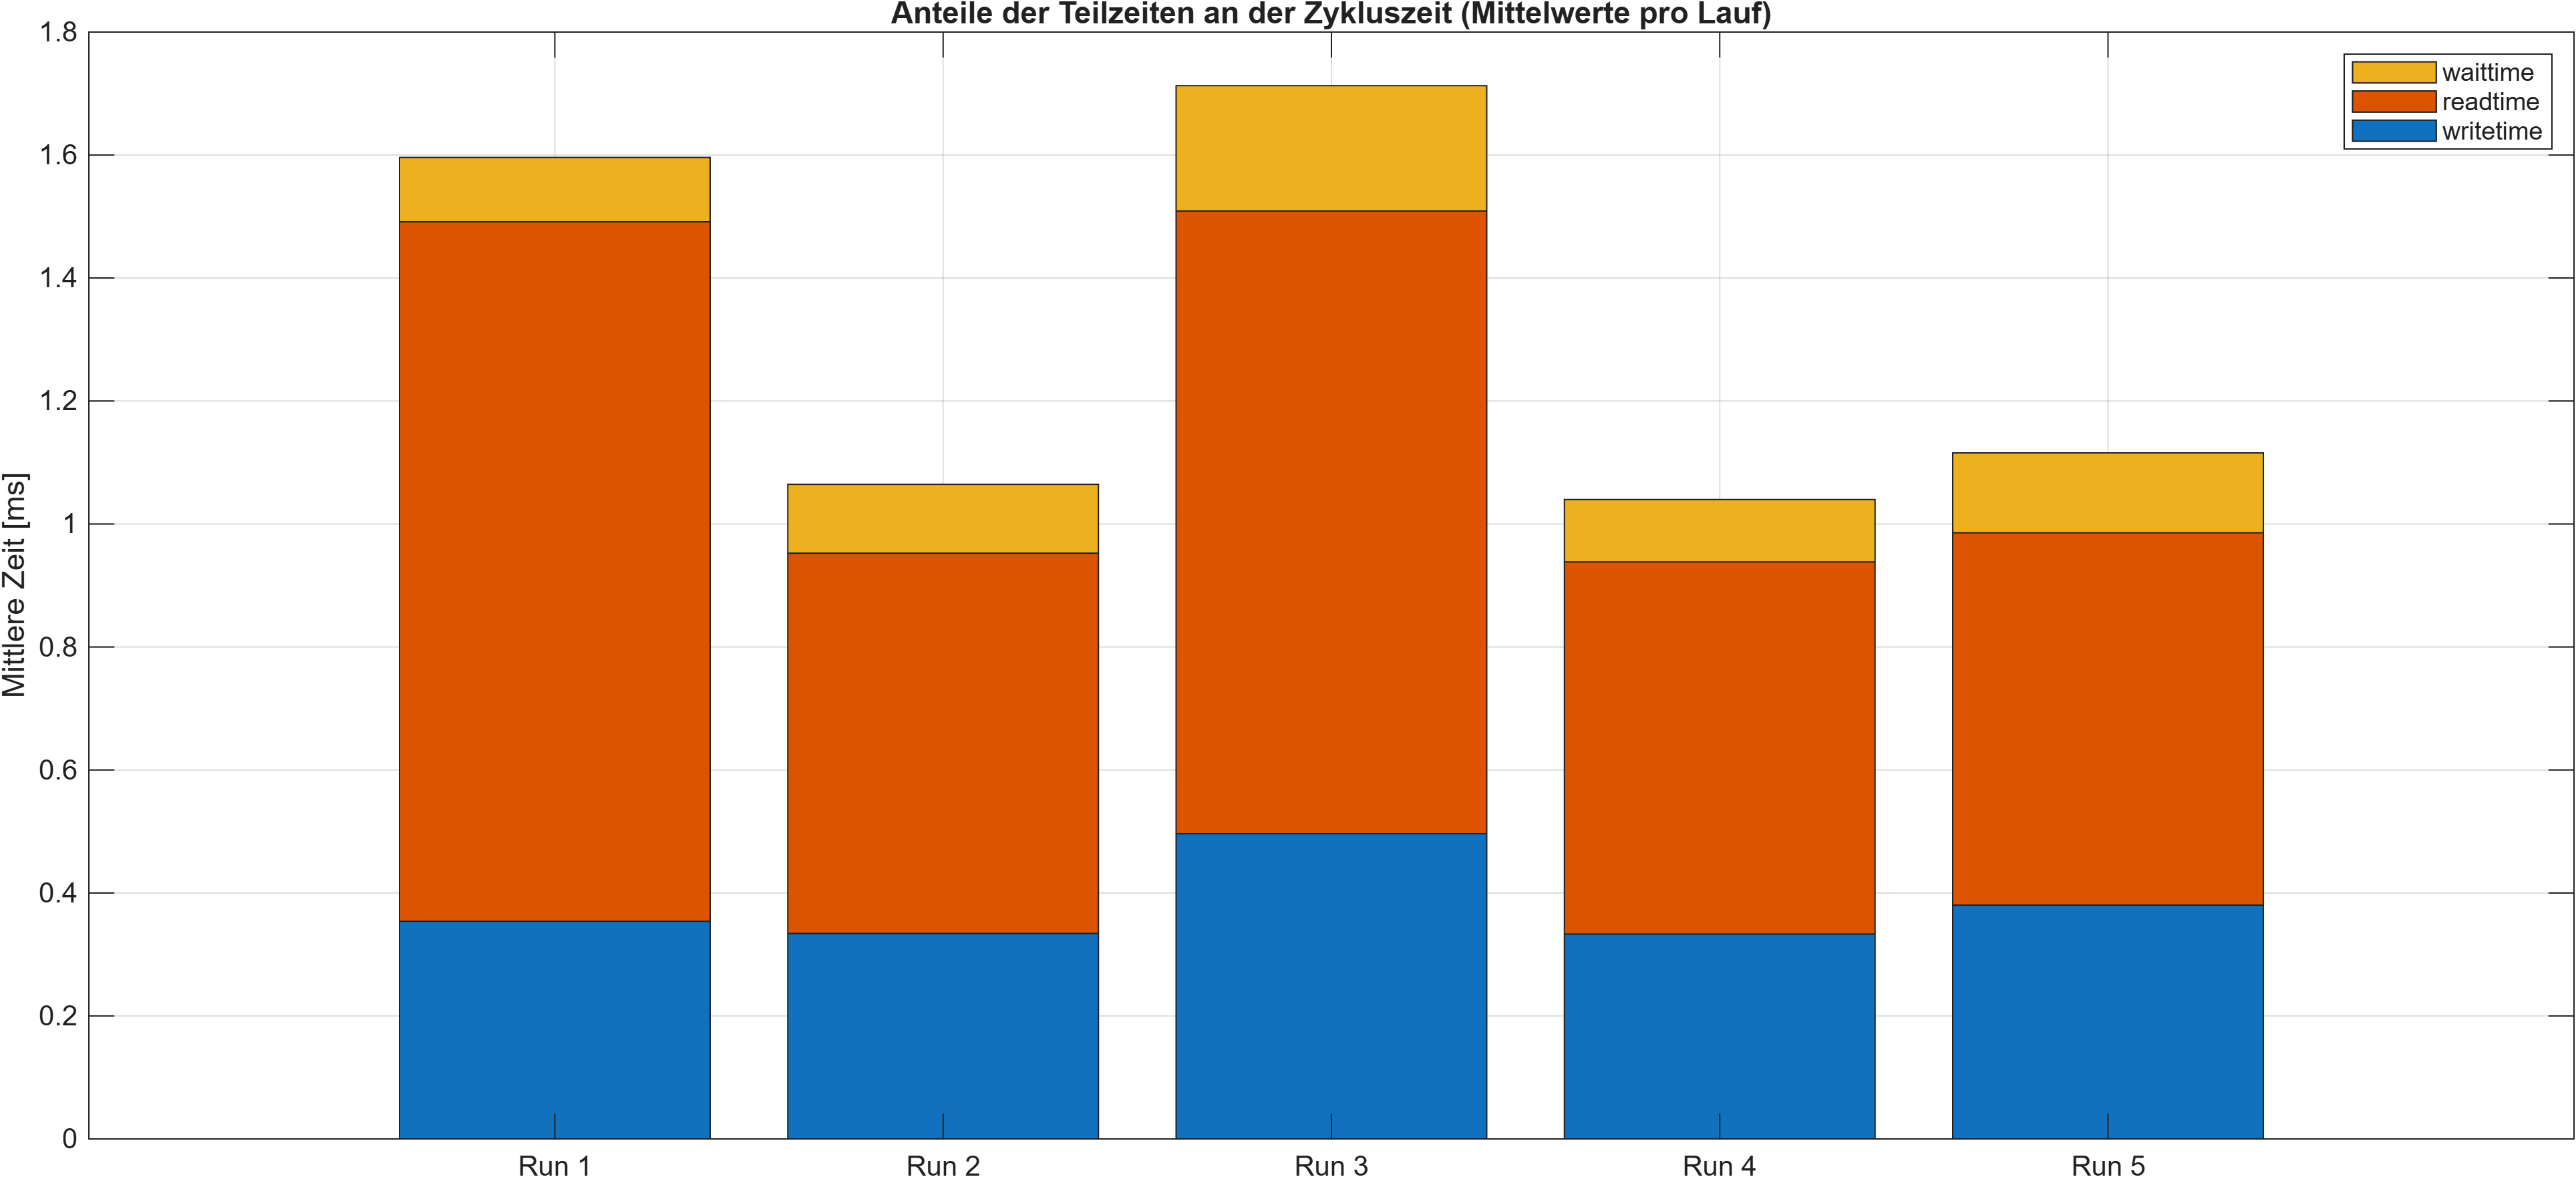
\includegraphics[width=0.75\linewidth]{images/teilzeiten_anteile.png}
    \caption{Mittlere Anteile der Teilzeiten an der Zykluszeit pro Lauf.}
    \label{fig:baseline_teilzeiten}
\end{figure}

Bei der Peak-Analyse lassen sich zwei Ursachen unterscheiden: Wiederkehrende
Spitzen von ca.\ \SIrange{65}{70}{\milli\second} treten in allen 5 Läufen an
denselben Zeitpunkten auf, die exakt mit den 4 Segmentübergängen der
Quadratbahn zusammenfallen: an diesen Stellen bleiben die gemessenen
Teilzeiten unauffällig klein, sodass die Verzögerung im MATLAB-Loop selbst
(Scheduling-Jitter) und nicht in der \ac{tcpip}-Kommunikation entsteht.
Vereinzelte Extremwerte (\SI{132}{\milli\second} in Run~1,
\SI{143}{\milli\second} in Run~3) zeigen sich dagegen direkt in
\texttt{polltime}/\texttt{readtime} und deuten auf echte, seltene
\ac{tcpip}-Aussetzer hin; ein Effekt, der auch mit einer deterministischen
QUARC-Anbindung nicht verschwinden wird, solange \ac{kvp}/Windows im
Kommunikationspfad verbleiben.

\subsubsection{Bahn-Genauigkeit}

Alle 5 Wegpunkte wurden in allen 5 Läufen innerhalb der Toleranz von
\SI{2.0}{\milli\meter} erreicht; die Restdistanz (\texttt{dmin}) an den
Zwischenpunkten (\SIrange{0.04}{0.05}{\milli\meter}) ist auf das aktivierte
Überschleifen (\texttt{CONT}, siehe Abschnitt~\ref{sec:krl}) zurückzuführen
und über alle 5 Läufe praktisch identisch (Abweichungen $< \SI{0.001}{\milli\meter}$).

\begin{figure}[H]
    \centering
    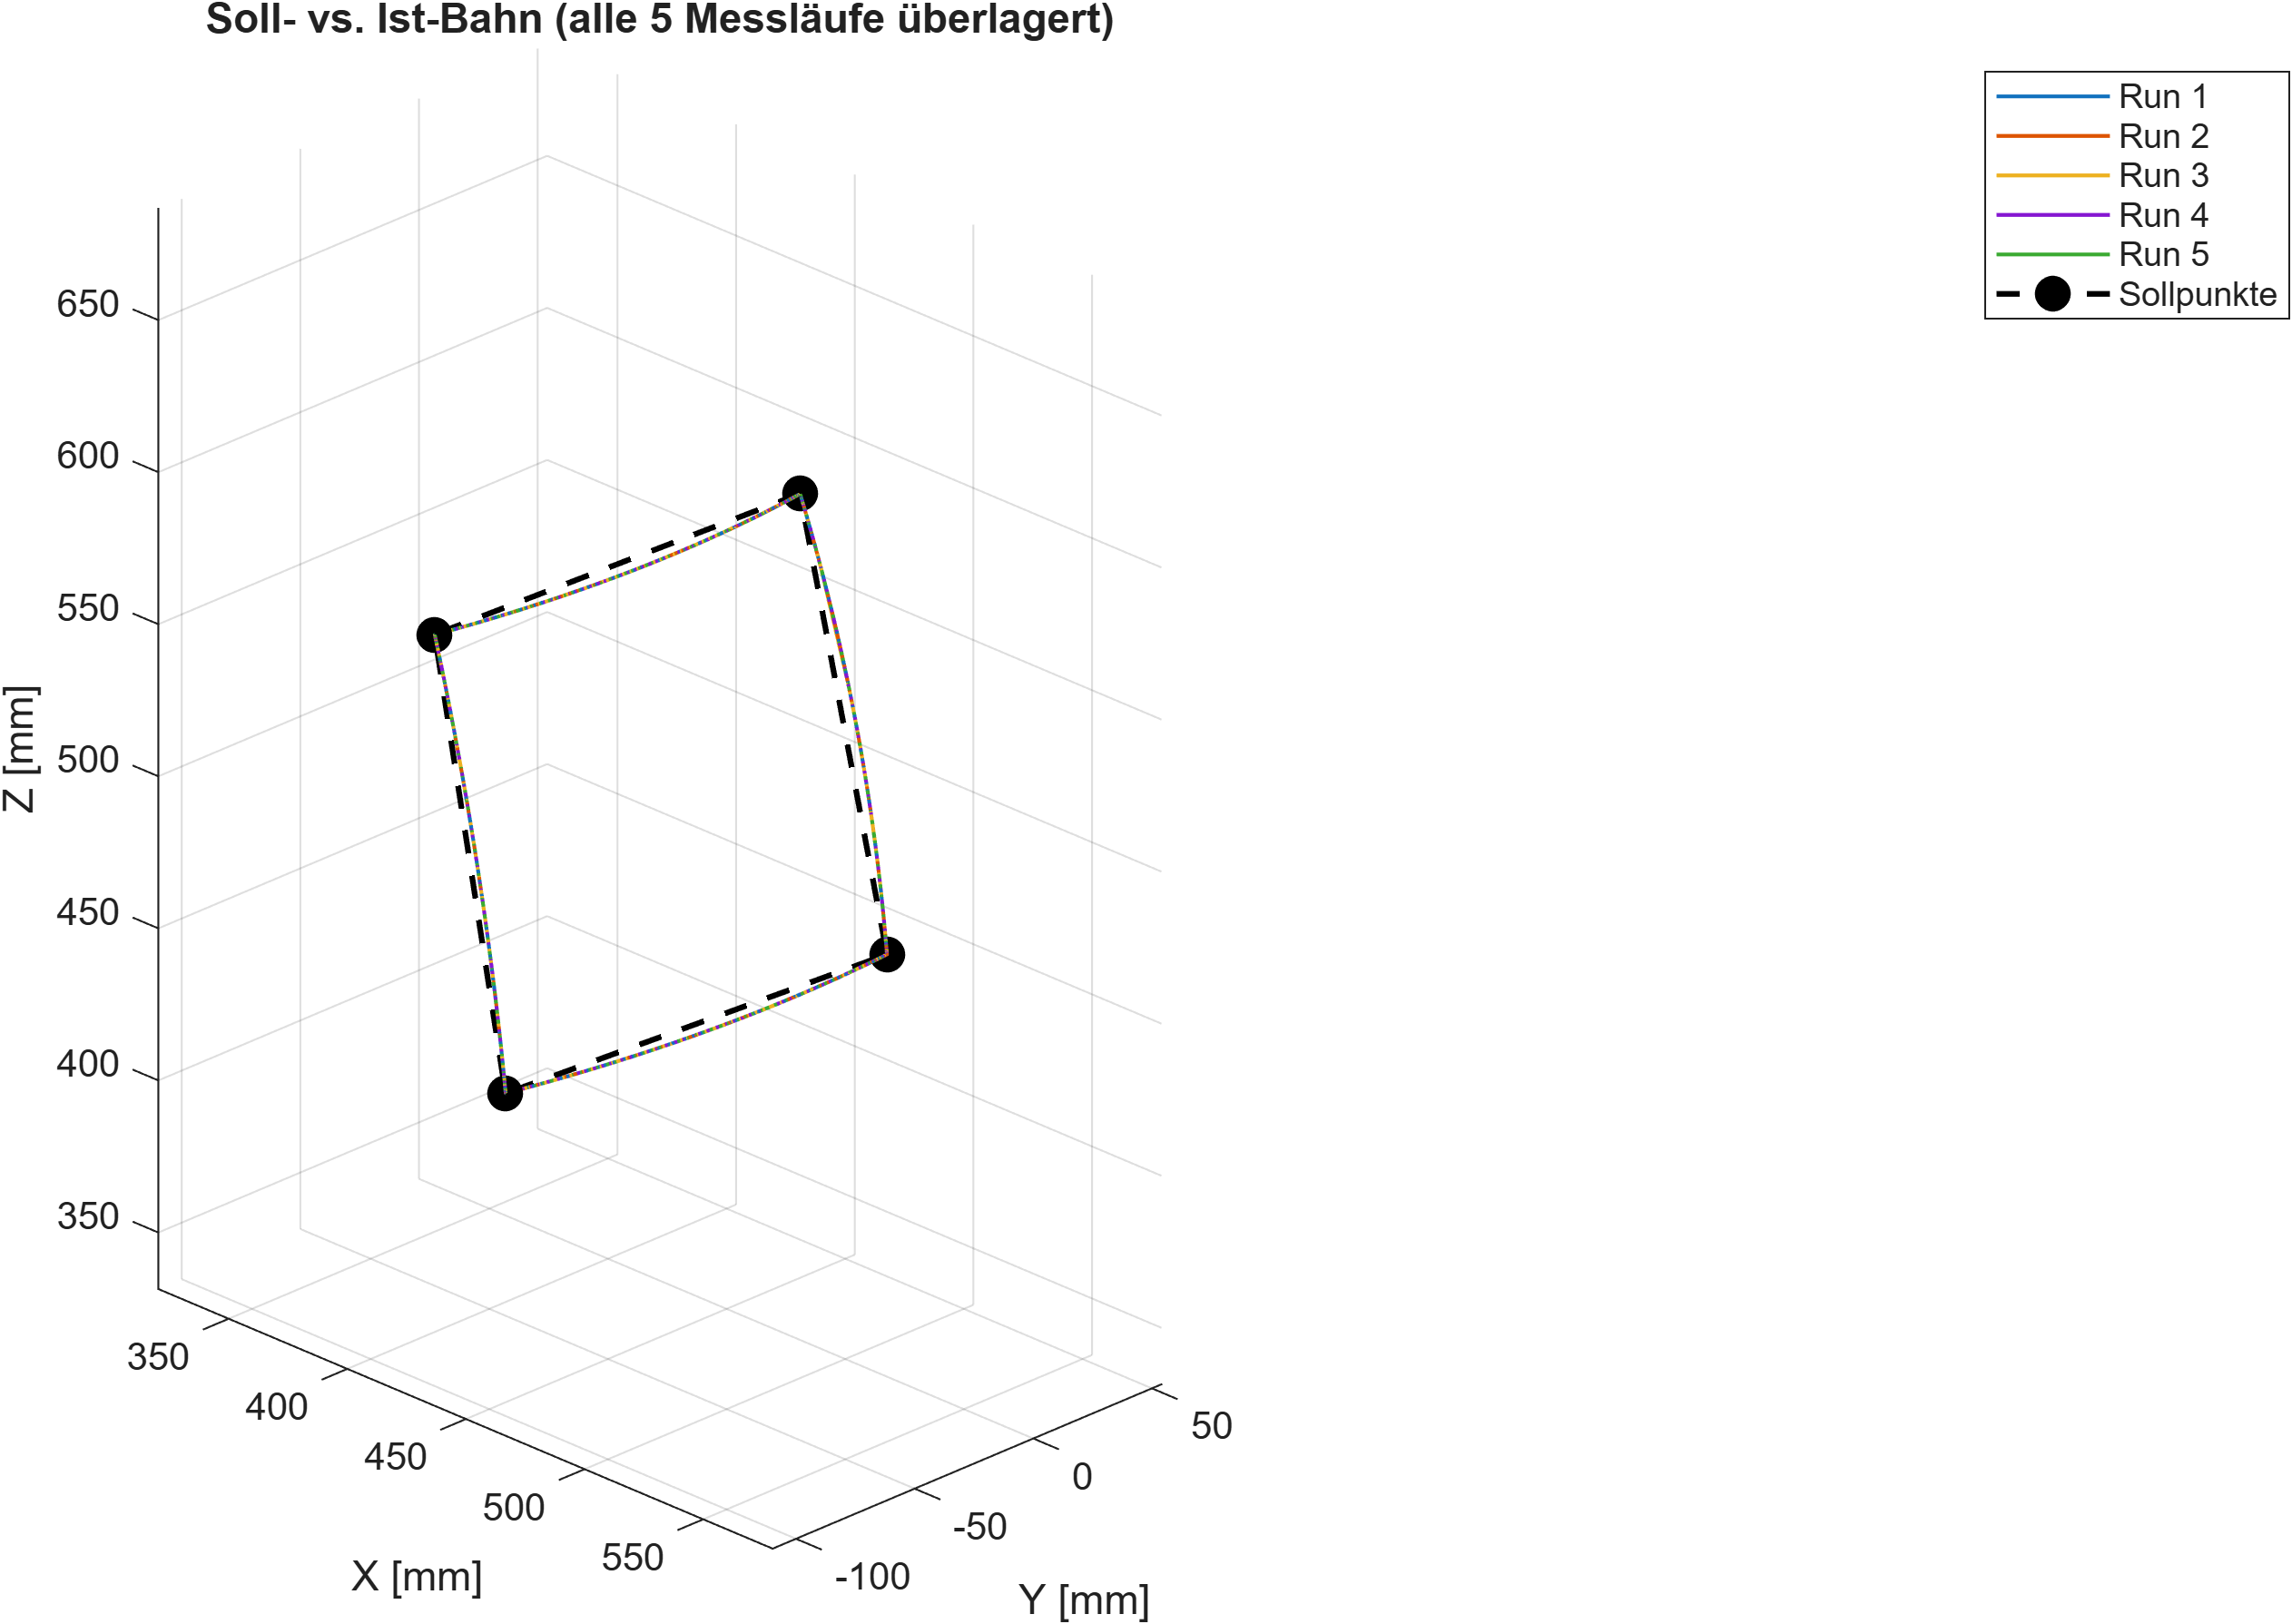
\includegraphics[width=0.8\linewidth]{images/soll_ist_bahn.png}
    \caption{Soll- und Ist-Bahn (alle 5 Messläufe überlagert).}
    \label{fig:baseline_bahn}
\end{figure}

\subsubsection{Einordnung als Baseline}

Zykluszeit-Verteilung, Teilzeiten-Aufschlüsselung, Peak-Ursachen und
Bahn-Genauigkeit dieser Messung bilden die MATLAB/KVP-Baseline aus
Anforderung~3 und dienen als Vergleichsmaßstab für die spätere
QUARC-Implementierung.

\subsection{Zykluszeitmessung der QUARC/Simulink-Anbindung}
\label{sec:quarc_zykluszeit}

Ergänzend zur MATLAB/KVP-Baseline (Abschnitt~\ref{sec:baseline}) wurde die
Zykluszeit-Zuverlässigkeit der neuen QUARC/Simulink-Anbindung untersucht.
Das verwendete Simulink-Modell (\texttt{SuR\_Projekt\_Wegpunkt\_v3.slx})
sendet die Bahnsollwerte PC-seitig deterministisch über den
QUARC-Echtzeitkern, wartet jedoch in dieser Ausbaustufe nicht auf eine
Rückmeldung des \ac{krl}-Programms auf der Steuerung (Pollen).
Die entsprechende Erweiterung war zum Zeitpunkt dieser Messung noch nicht
abgeschlossen.
Gemessen wurde daher zunächst nur, ob QUARC seinen eigenen
Modelltakt von \SI{100}{\milli\second} während der Laufzeit einhält.
Analog zur Baseline-Messung wurden dazu 5 identische Messläufe durchgeführt
(\texttt{QUARC\_Messung\_1}--\texttt{5.mat}). Ausgewertet wurden die
geloggten Signale \texttt{cycleTime\_QUARC}, \texttt{measurementActive\_QUARC}
und \texttt{time\_QUARC}, jeweils ohne den ersten Sample pro Lauf (kein
vollständiger Messzyklus). Auswertung und Abbildungen erzeugt das
MATLAB-Skript \texttt{auswertung\_quarc.m}, das die Struktur von
\texttt{auswertung\_baseline.m} übernimmt.
Anders als in dem Modell mit Sensor und Regelung werden hier nur die fünf Wegpunkte nach und nach vorgegeben und angefahren.
Ein generierter \ac{kvr}-Befehl kann dabei folgendermaßen aussehen:

\begin{lstlisting}
writeMsg = buildTargetMsg( ...
    420.1710, -93.1800, 574.0360, ...
    70.2850, 89.0000, 90.0000, ...
    2, 42);
\end{lstlisting}

Zur Erfassung des Modelltakts kann der Quanser Time-Block verwendet werden.
Die Schaltung hierfür ist in Abb.\ref{fig:timeblock} erkennbar.

\begin{figure}[H]
    \centering
    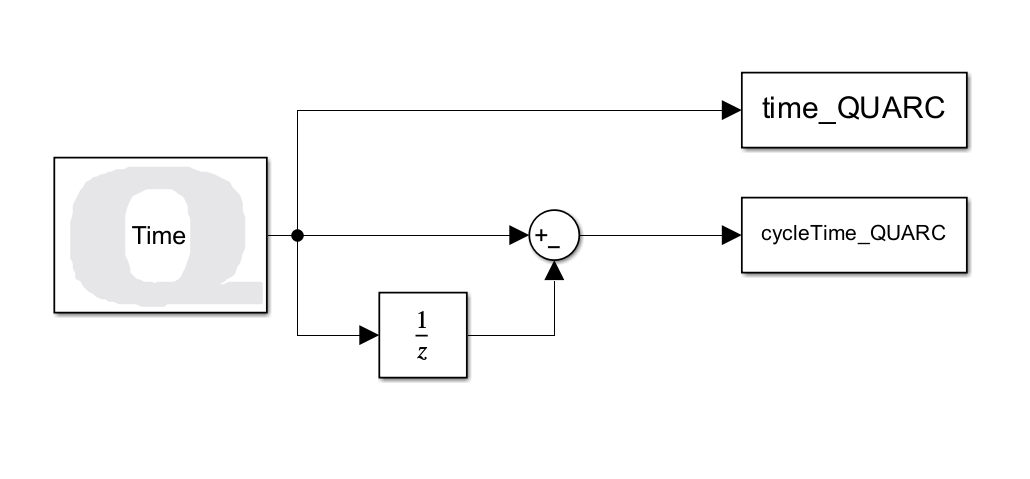
\includegraphics[width=0.8\linewidth]{images/quanserTime.png}
    \caption{Schaltung zur Takterfassung in Quanser}
    \label{fig:timeblock}
\end{figure}

Hiermit kann die Dauer jedes Takts erfasst werden.

\subsubsection{Zykluszeit}

Tabelle~\ref{tab:quarc_zykluszeit} zeigt die Zykluszeit-Statistik pro Lauf
sowie gepoolt über alle 1152 gültigen Samples.

\begin{table}[H]
    \centering
    \caption{Zykluszeit-Statistik der QUARC-Anbindung in
    \si{\milli\second} (aus \texttt{cycleTime\_quarc\_stats.csv}).}
    \label{tab:quarc_zykluszeit}
    \begin{tabular}{lrrrrrrr}
        \toprule
        Lauf & $n$ & MW & Median & StdAbw & Min & Max & P95 \\
        \midrule
        Run 1 & 291 & 99.998  & 99.962 & 0.415 & 99.045 & 100.950 & 100.712 \\
        Run 2 & 222 & 100.002 & 99.982 & 0.408 & 98.809 & 101.358 & 100.676 \\
        Run 3 & 215 & 99.997  & 99.970 & 0.382 & 99.075 & 100.860 & 100.600 \\
        Run 4 & 242 & 100.003 & 99.979 & 0.410 & 99.140 & 100.988 & 100.656 \\
        Run 5 & 182 & 100.001 & 99.970 & 0.393 & 99.080 & 100.816 & 100.647 \\
        \midrule
        Gesamt (gepoolt) & 1152 & \textbf{100.000} & \textbf{99.972} & 0.402 & 98.809 & 101.358 & 100.657 \\
        \bottomrule
    \end{tabular}
\end{table}

QUARC hält den \SI{100}{\milli\second}-Modelltakt praktisch exakt ein: Der
gepoolte Mittelwert liegt bei genau \SI{100.000}{\milli\second}, die
Standardabweichung bei nur \SI{0.40}{\milli\second} (\SI{0.4}{\percent} des
Sollwerts). Der größte Ausreißer über alle 5 Läufe weicht \SI{1.36}{\milli\second}
vom Soll ab; kein einziger der 1152 Samples überschreitet
\SI{1.4}{\milli\second} Abweichung.

\begin{figure}[H]
    \centering
    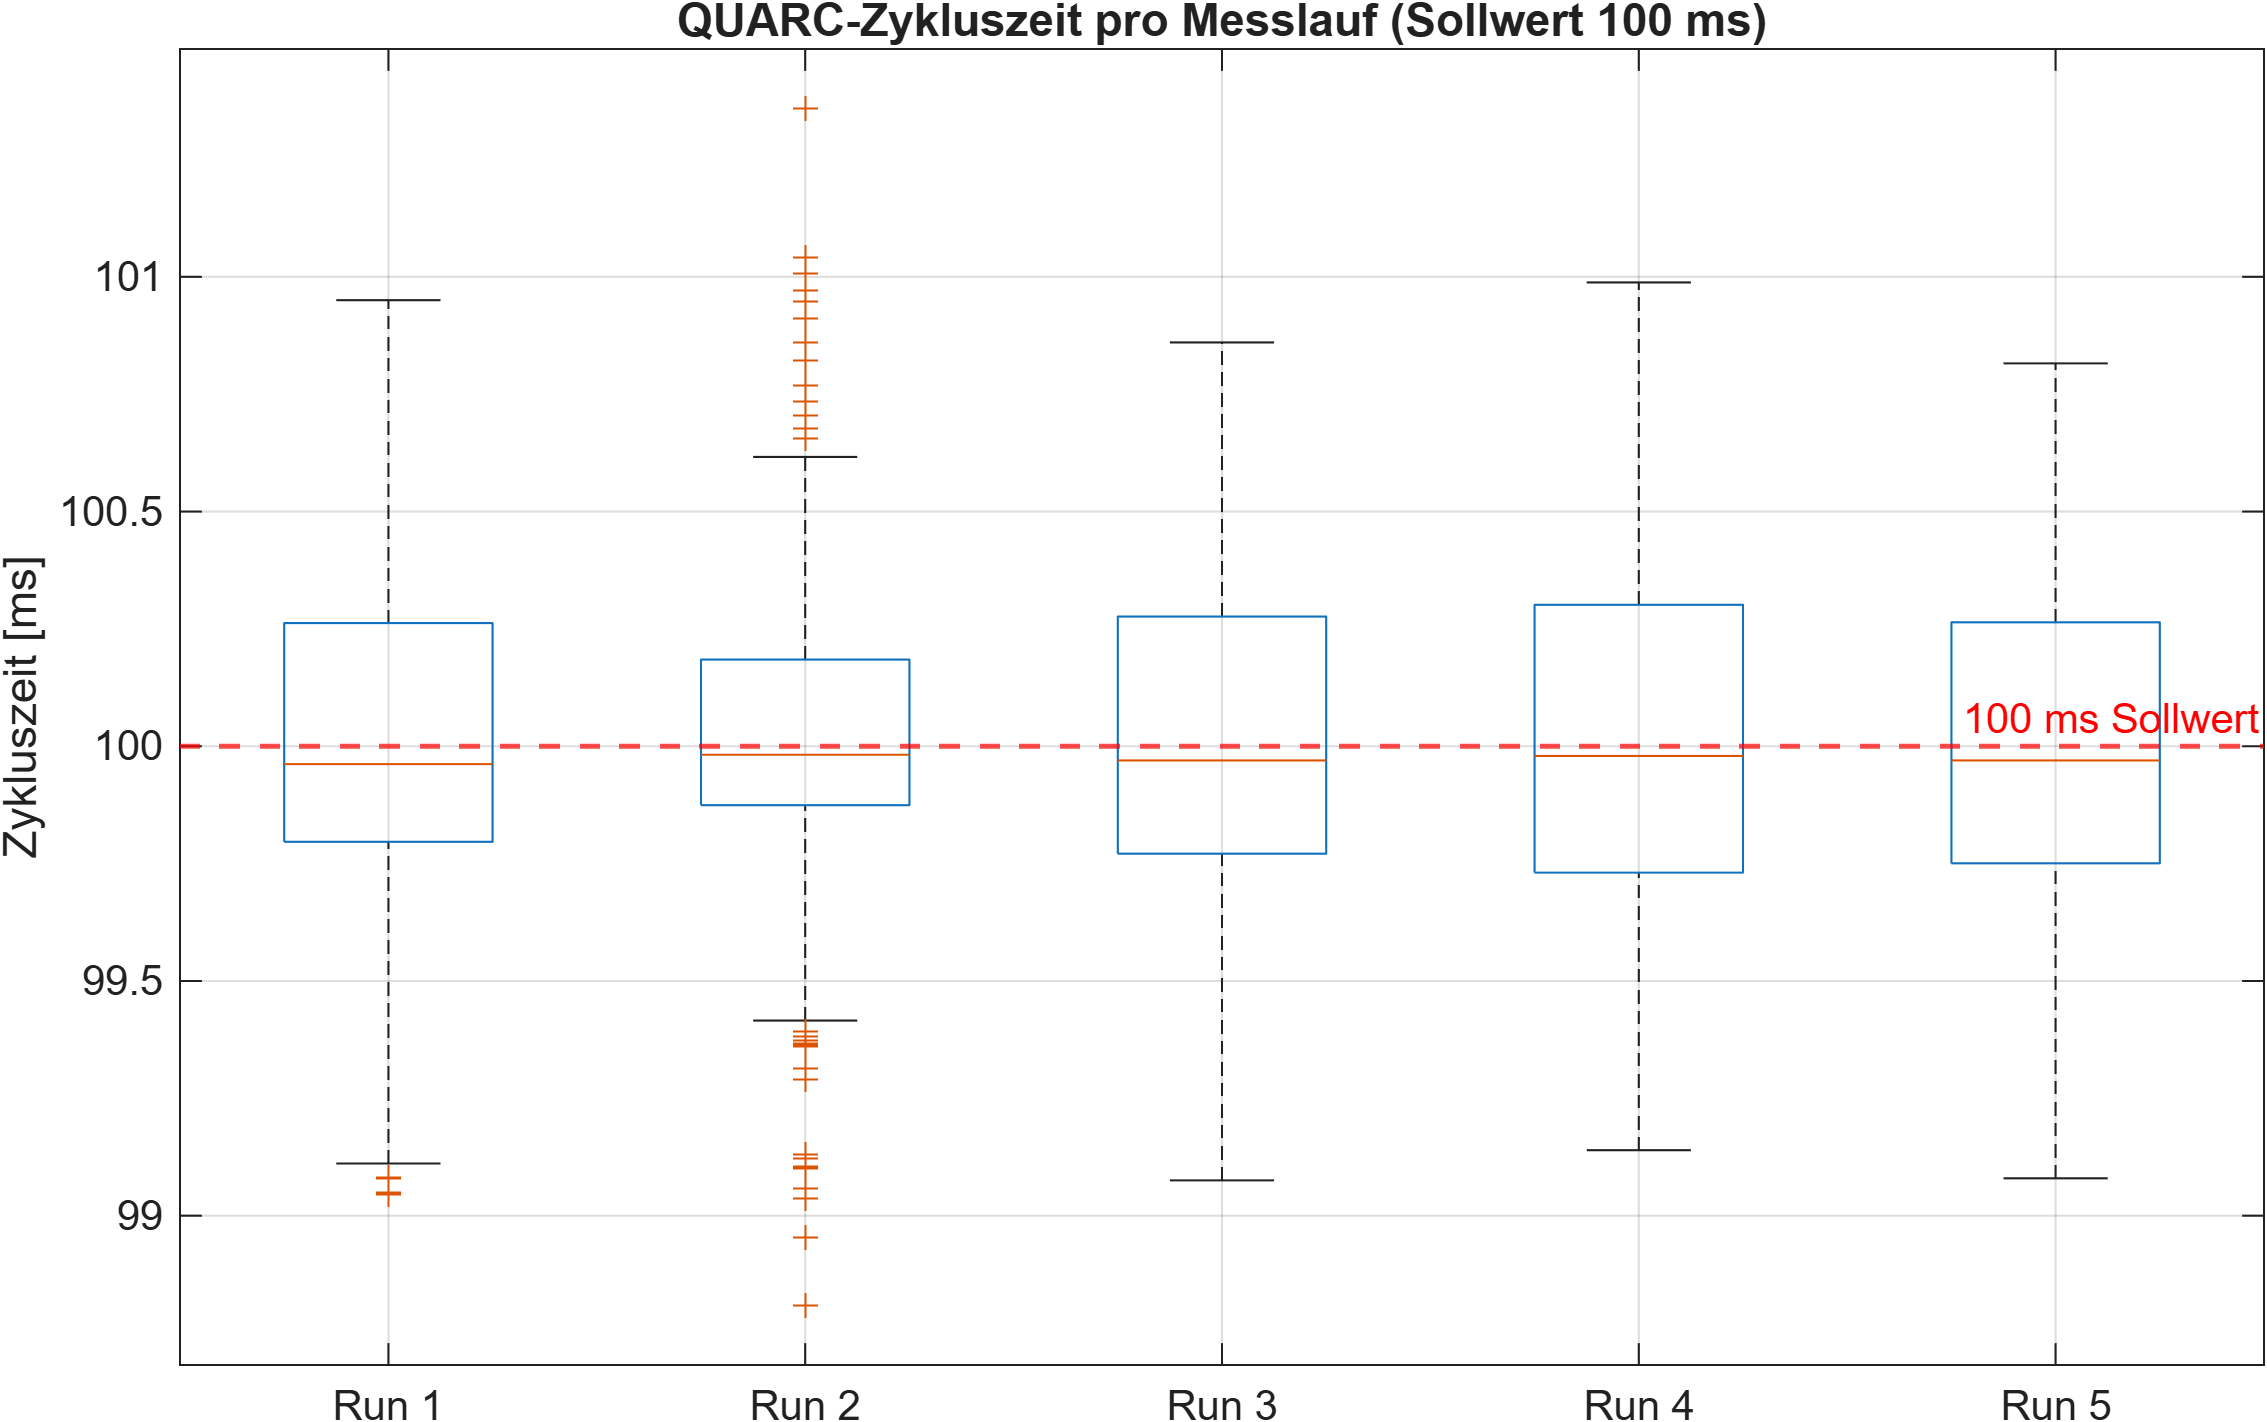
\includegraphics[width=0.75\linewidth]{images/quarc_zykluszeit_boxplot.png}
    \caption{QUARC-Zykluszeit pro Messlauf (Boxplot) mit
    \SI{100}{\milli\second}-Referenzlinie, erzeugt mit
    \texttt{auswertung\_quarc.m}.}
    \label{fig:quarc_boxplot}
\end{figure}

\begin{figure}[H]
    \centering
    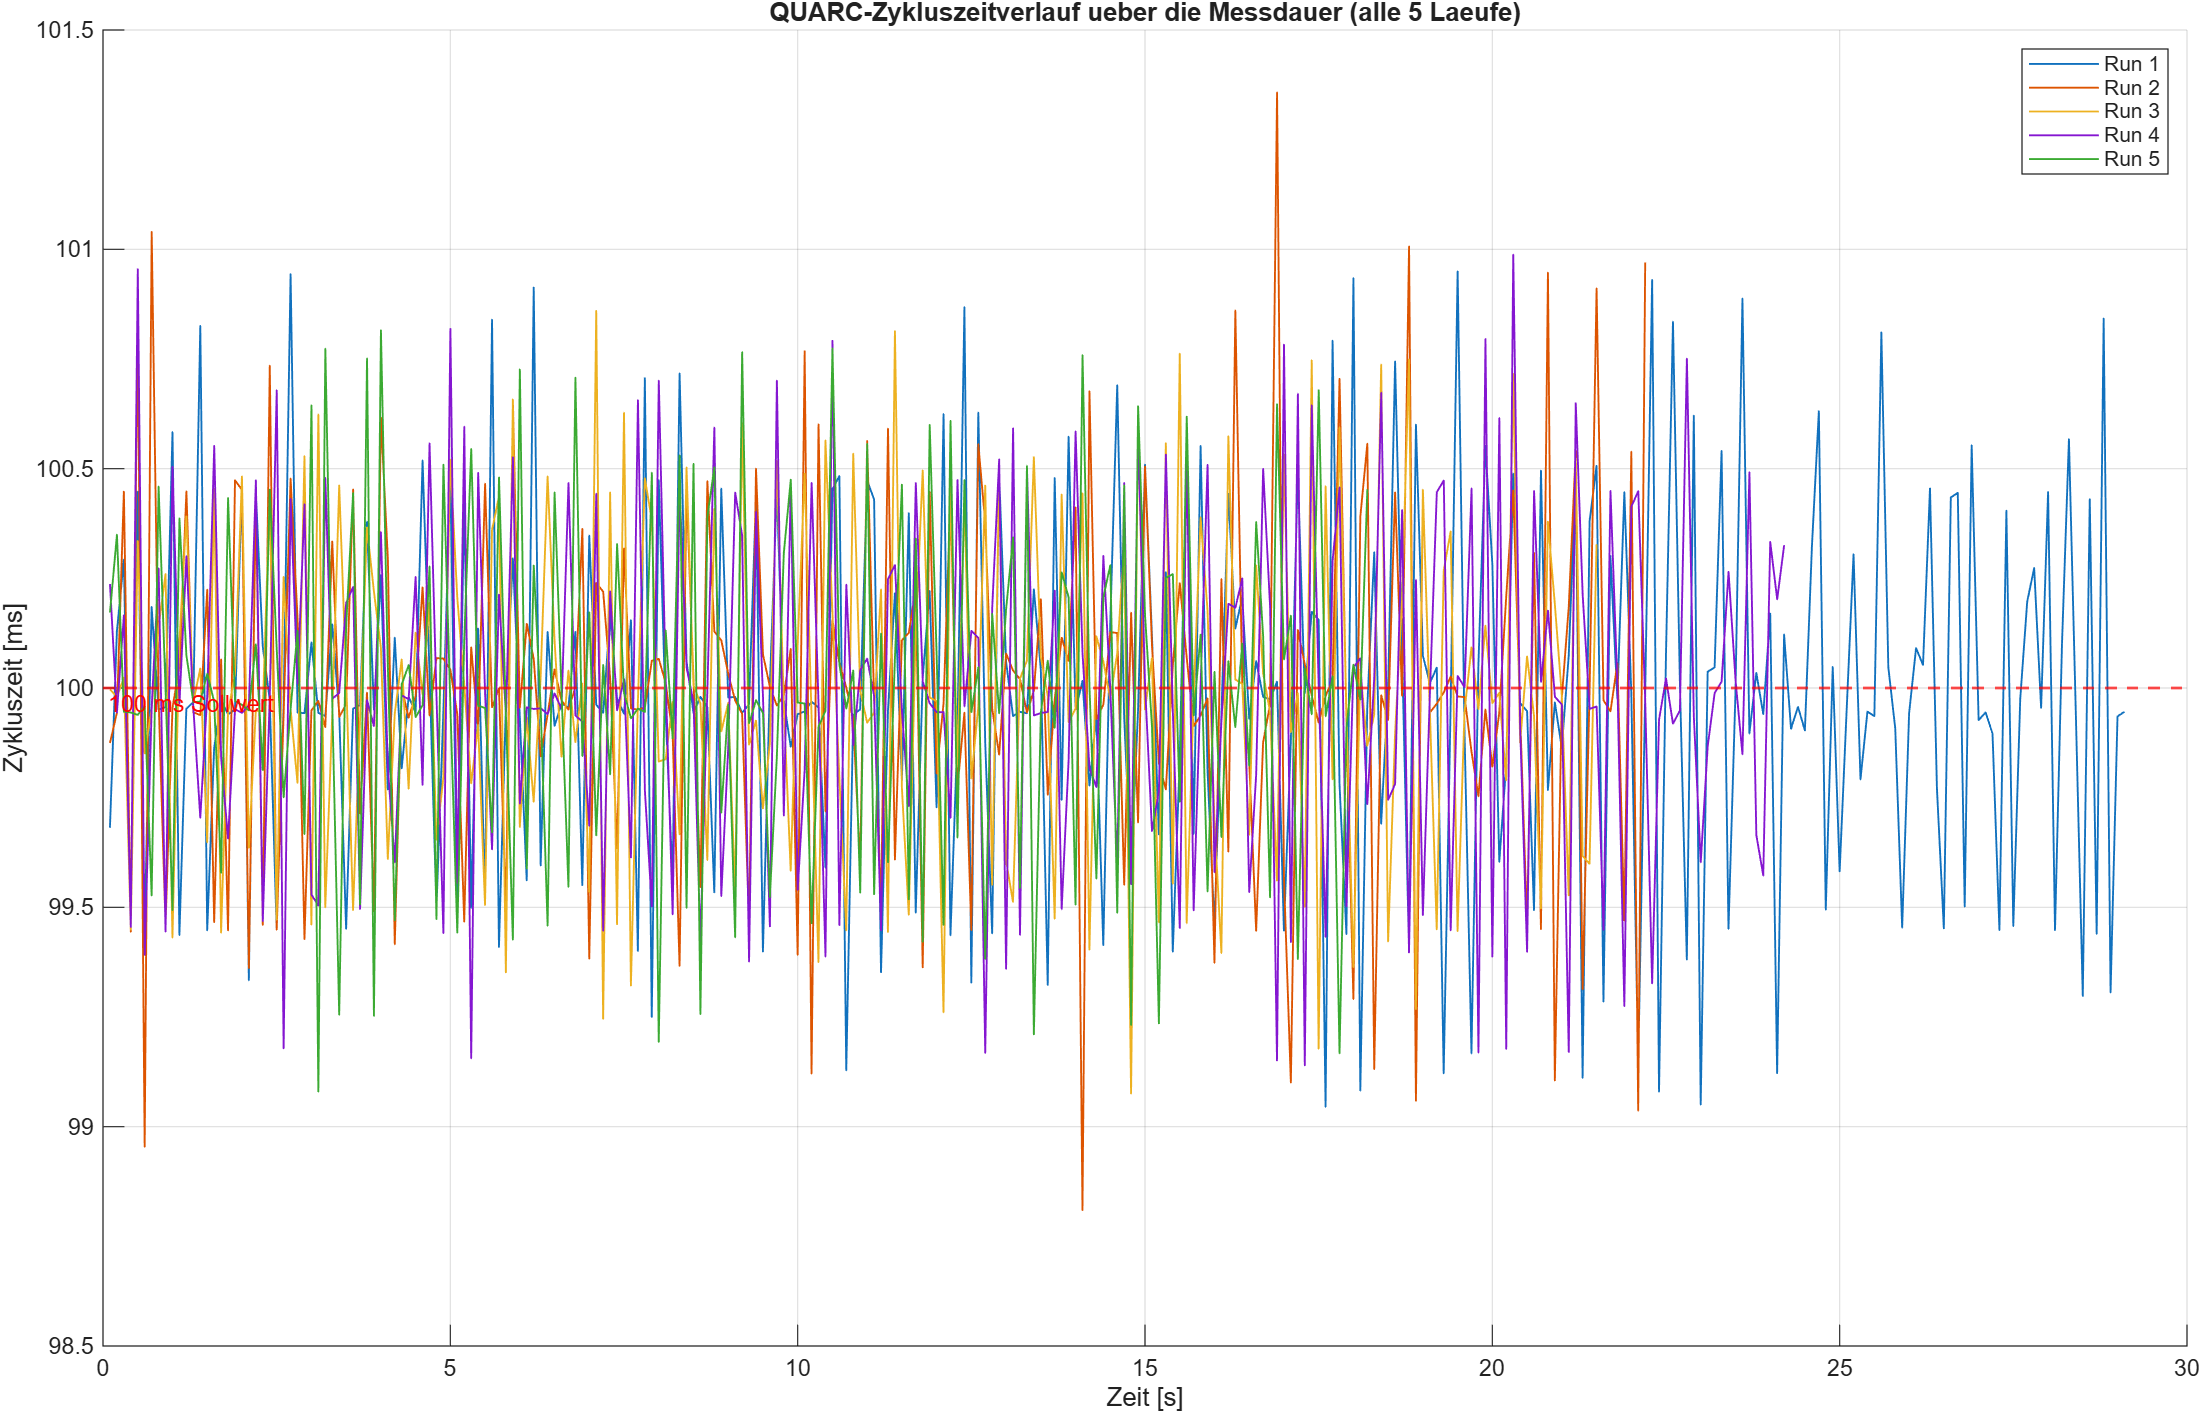
\includegraphics[width=0.9\linewidth]{images/quarc_zykluszeit_zeitverlauf.png}
    \caption{Zeitverlauf der Zykluszeit über alle 5 Läufe, mit
    \SI{100}{\milli\second}-Referenzlinie.}
    \label{fig:quarc_zeitverlauf}
\end{figure}

\subsubsection{Vergleich zur MATLAB/KVP-Baseline}

Tabelle~\ref{tab:vergleich_kvp_quarc} stellt die Zykluszeit-Zuverlässigkeit
beider Anbindungen gegenüber (jeweils relativ zum eigenen Sollwert, da
\ac{krl} mit \SI{12}{\milli\second} und QUARC mit \SI{100}{\milli\second}
takten).

\begin{table}[H]
    \centering
    \caption{Vergleich der Zykluszeit-Zuverlässigkeit: MATLAB/KVP-Baseline
    vs.\ QUARC.}
    \label{tab:vergleich_kvp_quarc}
    \begin{tabular}{lrr}
        \toprule
        Größe & MATLAB/KVP (Soll \SI{12}{\milli\second}) & QUARC (Soll \SI{100}{\milli\second}) \\
        \midrule
        Mittelwert vs.\ Soll & +\SI{5.27}{\milli\second} (+\SI{43.9}{\percent}) & +\SI{0.0004}{\milli\second} ($\pm\SI{0.0}{\percent}$) \\
        Median & \SI{16.6}{\milli\second} & \SI{99.97}{\milli\second} \\
        Std.-Abw. & \SI{6.18}{\milli\second} (\SI{51}{\percent} des Solls) & \SI{0.40}{\milli\second} (\SI{0.4}{\percent} des Solls) \\
        Max.\ Abweichung & +\SI{130.8}{\milli\second} (Ausreißer) & +\SI{1.36}{\milli\second} \\
        \bottomrule
    \end{tabular}
\end{table}

Das entspricht dem in Anforderung~1 erwarteten Effekt: Über QUARCs
Echtzeitkern sendet die PC-Seite ihre Daten deterministisch, unabhängig vom
MATLAB-Interpreter-Overhead, der die alte Anbindung dominiert hat. Die
verbleibende Streuung von $\pm\SI{1.4}{\milli\second}$ liegt im Bereich
dessen, was von einem Soft-/Hard-Realtime-Ziel unter Simulink External Mode
zu erwarten ist.

\subsubsection{Peak-Analyse und Bahnzeit-Konsistenz}

Anders als bei der Baseline-Messung, wo die größten Abweichungen exakt an
den 4 Bahnsegmentübergängen auftraten (Abschnitt~\ref{sec:baseline_teilzeiten}),
zeigen die größten Abweichungen bei QUARC \textbf{kein} erkennbares Muster:
Sie treten zu unterschiedlichen Zeitpunkten je Lauf auf, sind mal positiv,
mal negativ, und liegen alle unter \SI{1.4}{\milli\second}. Auch zwischen
aktiver Messphase (\texttt{measurementActive = 1}) und Vor-/Nachlauf zeigt
sich kein messbarer Unterschied in Mittelwert oder Streuung: das Modell
taktet durchgehend gleich.

\begin{figure}[H]
    \centering
    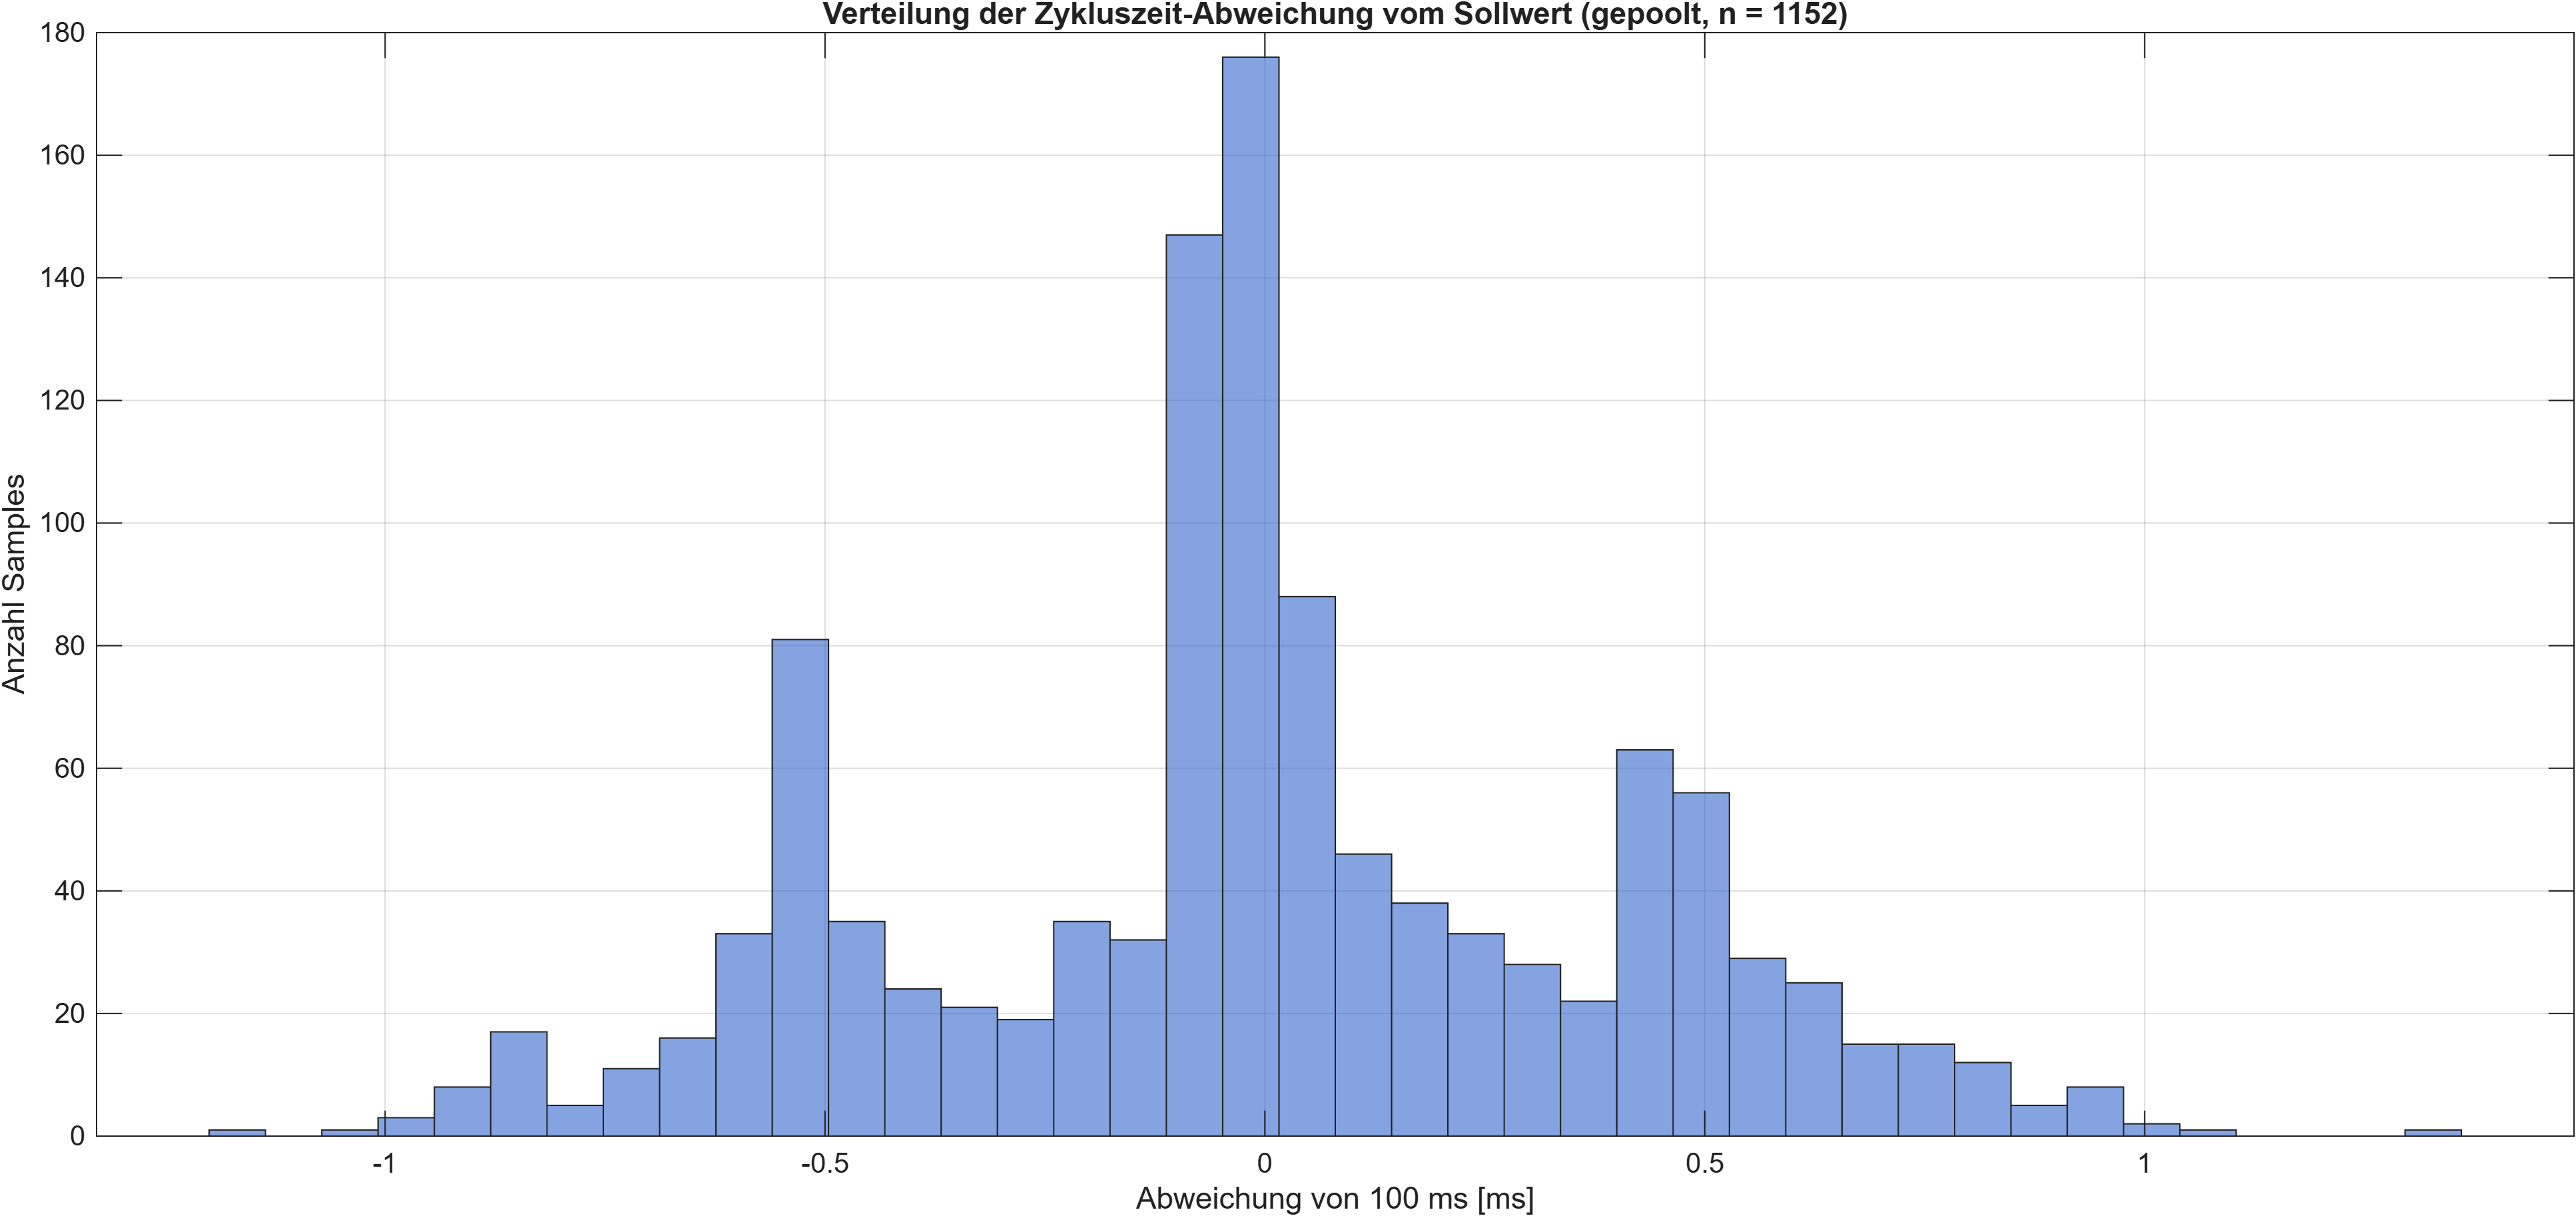
\includegraphics[width=0.75\linewidth]{images/quarc_abweichung_histogramm.png}
    \caption{Verteilung der Zykluszeit-Abweichung vom Sollwert, gepoolt über
    alle 5 Läufe ($n = 1152$).}
    \label{fig:quarc_histogramm}
\end{figure}

Die aktive Messphase (\texttt{measurementActive = 1}) ist in allen 5 Läufen
exakt 119 Samples lang und dauert praktisch identisch \SI{11.80}{\second}
(Streuung $< \SI{0.5}{\milli\second}$ zwischen den Läufen), obwohl sich die
Gesamtlänge der 5 \texttt{.mat}-Dateien stark unterscheidet
(182--291 Samples). Die unterschiedliche Gesamtlänge stammt somit allein aus
unterschiedlich langem Vor-/Nachlauf bei Aufnahmestart bzw.\ -stopp, nicht
aus einer unterschiedlichen Bahn oder Geschwindigkeit; ein gutes Zeichen
für die Reproduzierbarkeit des QUARC-Aufbaus.

\begin{figure}[H]
    \centering
    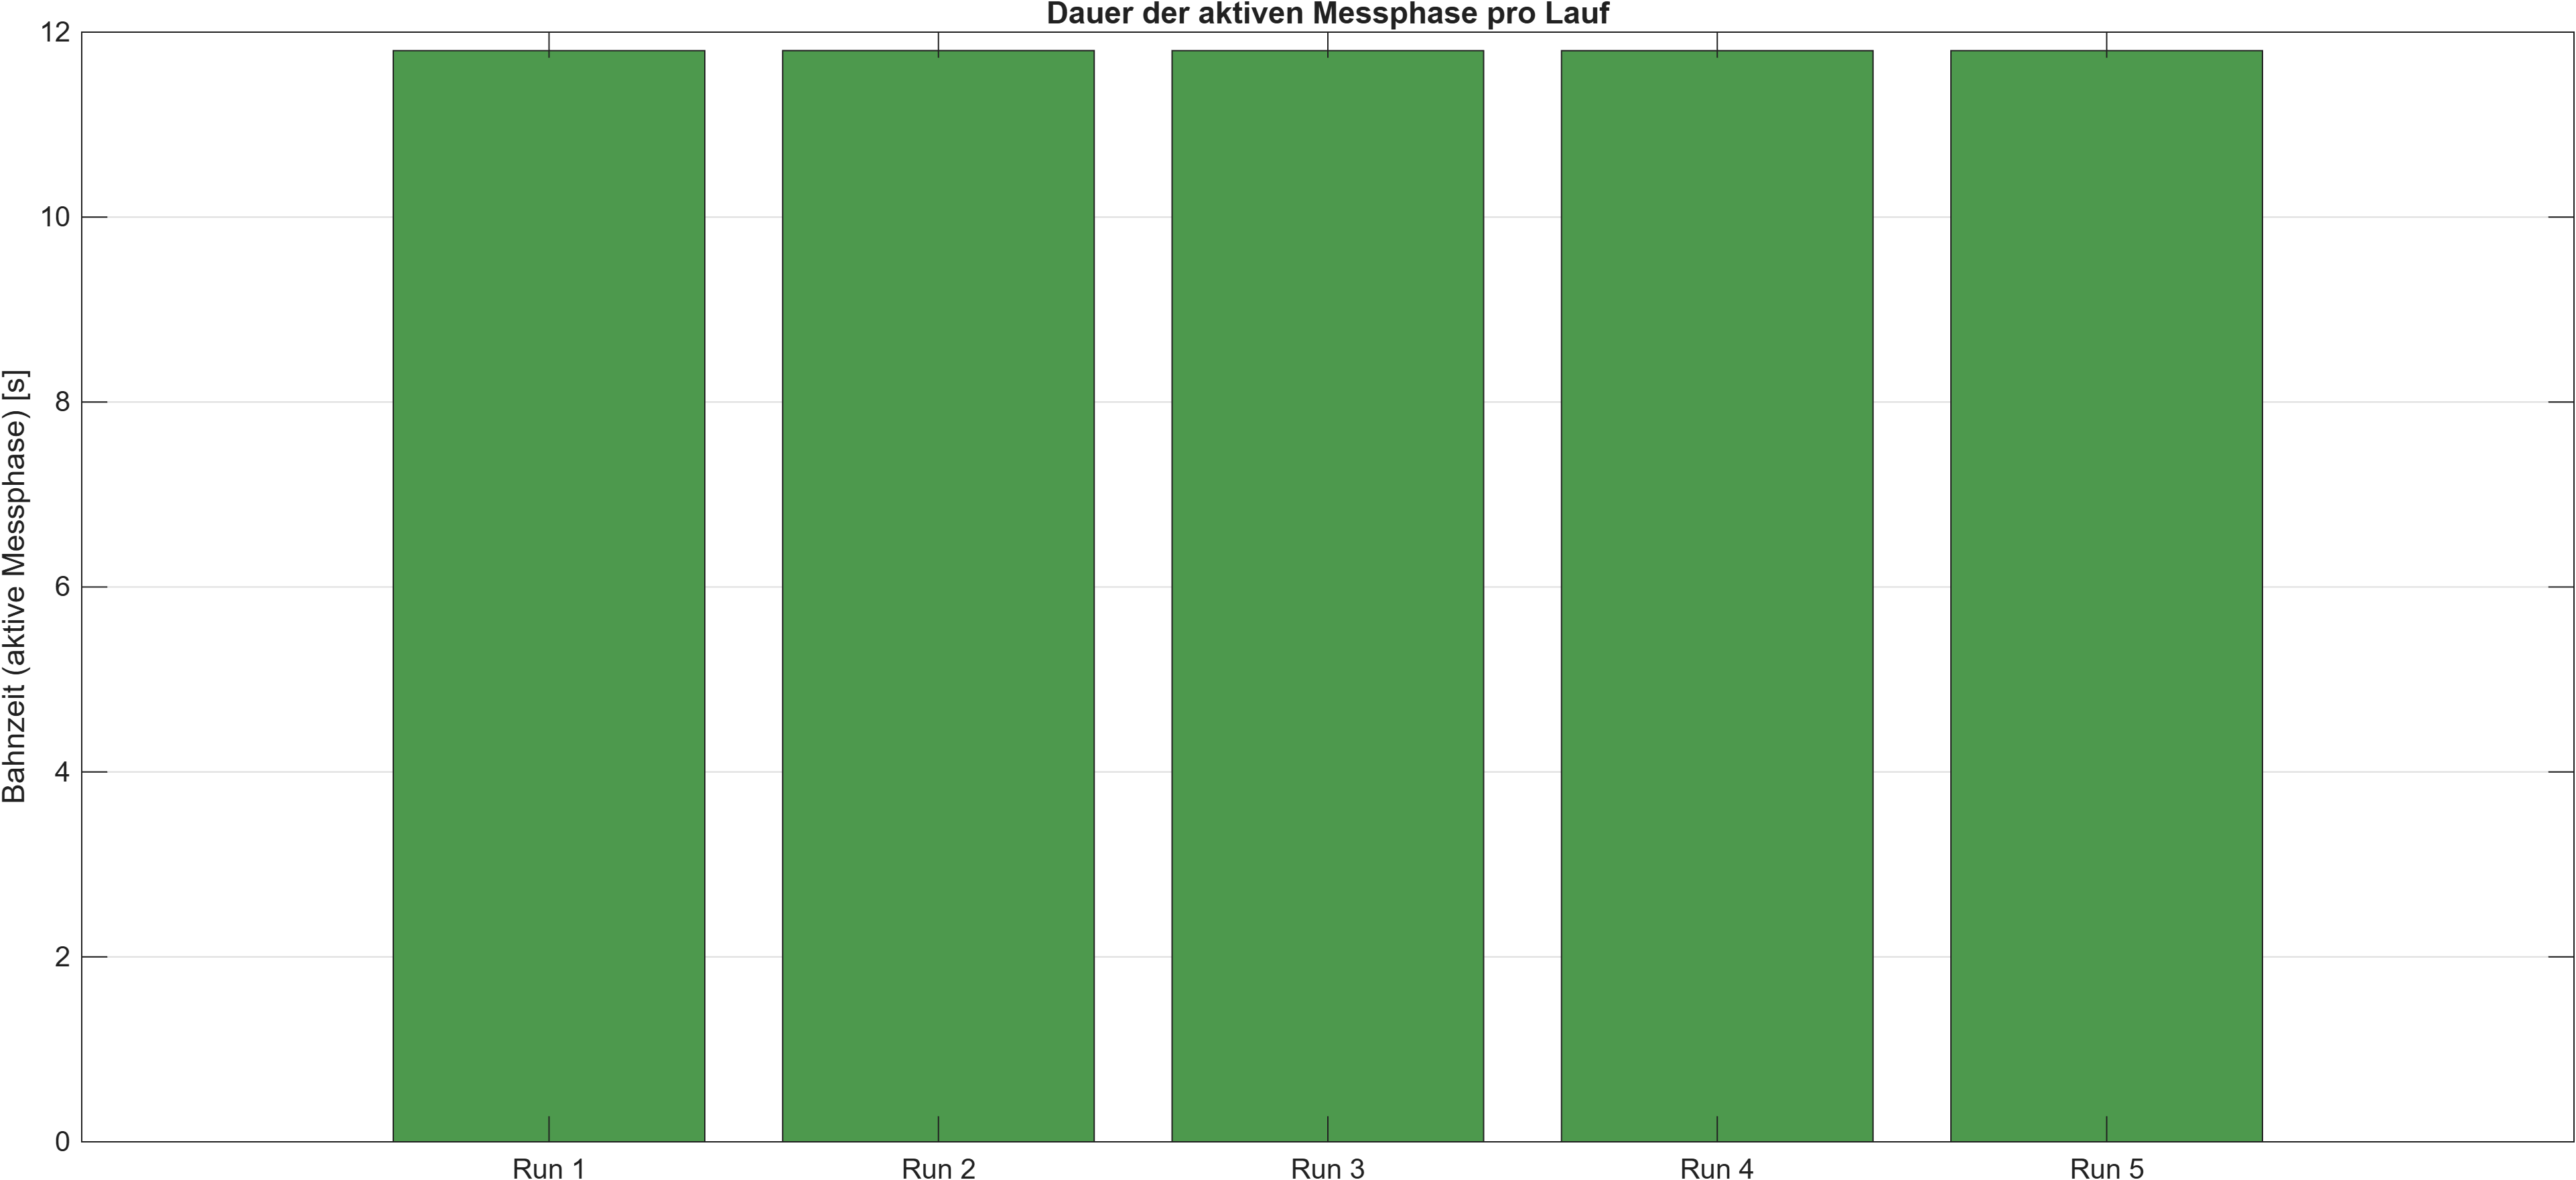
\includegraphics[width=0.75\linewidth]{images/quarc_bahnzeit.png}
    \caption{Dauer der aktiven Messphase (Bahnzeit) pro Lauf.}
    \label{fig:quarc_bahnzeit}
\end{figure}

\subsubsection{Einordnung und offene Punkte}

Diese Messung zeigt, wie zuverlässig QUARC selbst seinen
\SI{100}{\milli\second}-Modelltakt PC-seitig einhält. Sie erfasst jedoch noch
nicht die Ende-zu-Ende-Latenz zum \ac{krl}-Programm auf der Steuerung, also
ob und wie schnell der Roboter tatsächlich auf ein gesendetes Sollsignal
reagiert bzw.\ wie lange eine Positions-Rückmeldung braucht. Für
Anforderung~3 ist das PC-seitige Timing damit ein notwendiger, aber noch
nicht hinreichender Baustein; die vollständige Ende-zu-Ende-Messung setzt
die noch ausstehende Polling-Implementierung auf QUARC-Seite voraus.

\subsection{QUARC-Portierung, Sensor-Integration und Regelungsapplikation}

\subsection{Regelungsversuche und Bewertung (?)}
Zur ersten Charakterisierung der Regelstrecke mit dem realen
Ultraschallsensor wurde ein Sprungversuch durchgeführt: Der
Distanz-Sollwert (\texttt{soll}) wird bei $t=\SI{10.8}{\second}$ sprunghaft
von \SI{30}{\centi\meter} auf \SI{20}{\centi\meter} reduziert, während die
Robotersteuerung parallel den zugehörigen Positionsbefehl (\texttt{Target})
sowie die tatsächliche Roboterposition (\texttt{istPosition}) in
Millimeter mitschreibt. Abbildung~\ref{fig:realsensor_gesamt} zeigt alle
fünf aufgezeichneten Signale überlagert, Abbildung~\ref{fig:realsensor_einzeln}
dieselben Daten als Einzelplots.

\begin{figure}[H]
    \centering
    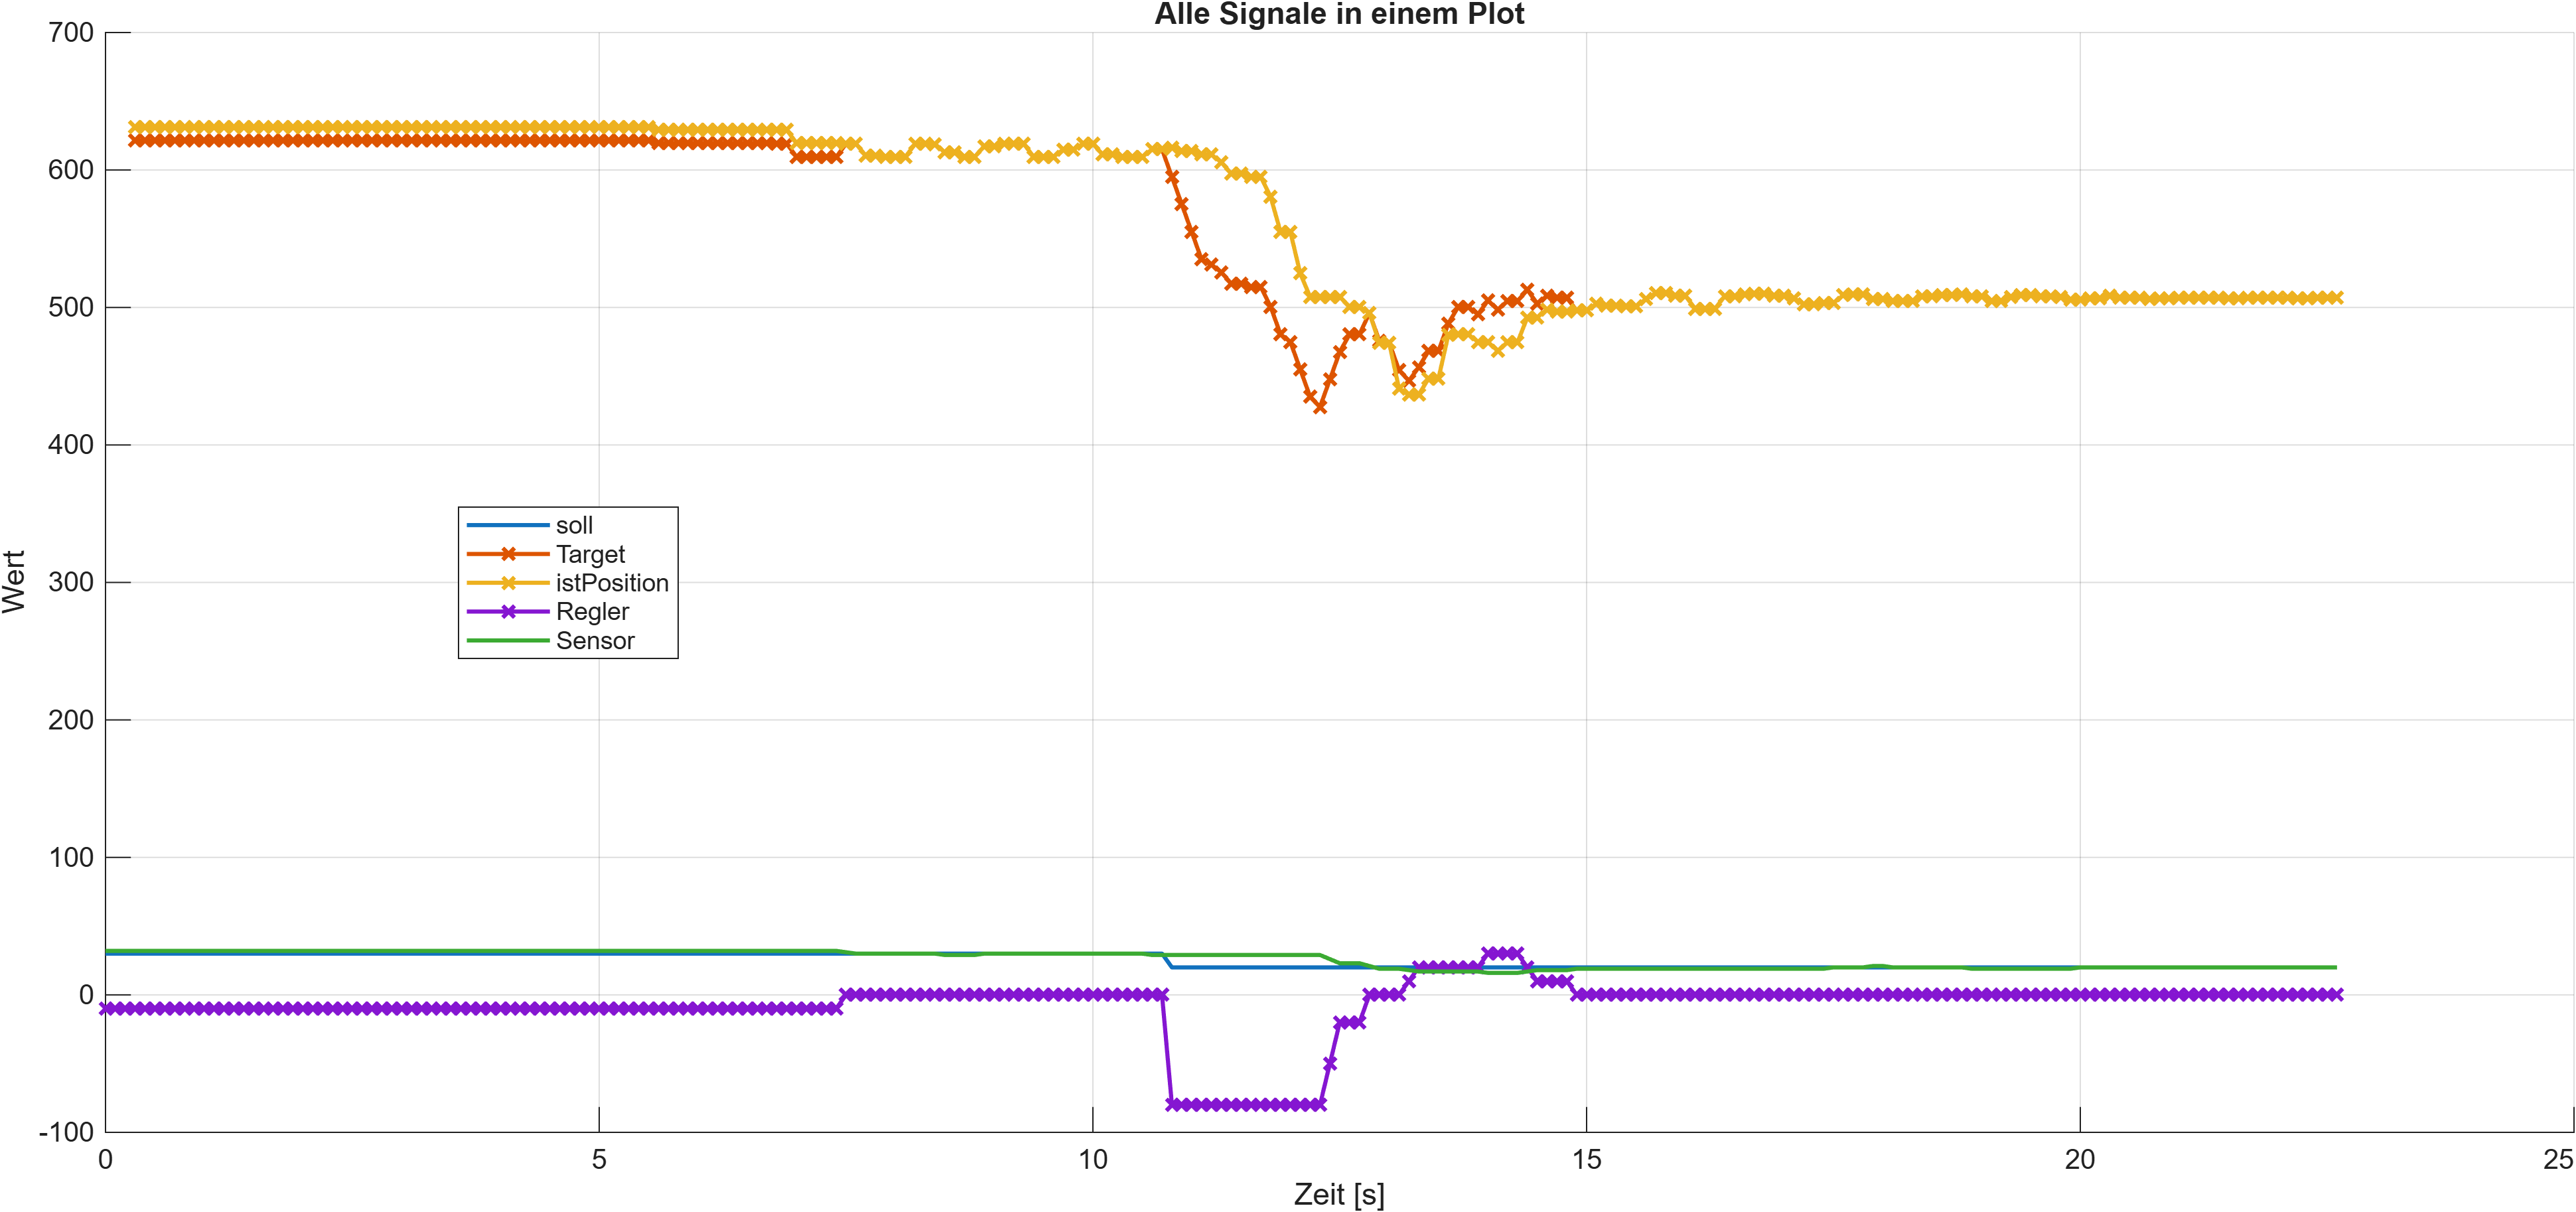
\includegraphics[width=0.85\linewidth]{images/realsensor_signale_gesamt.png}
    \caption{Sprungversuch am realen Ultraschallsensor: alle Signale
    überlagert, erzeugt mit \texttt{Auswertung\_RealSensor.m}.}
    \label{fig:realsensor_gesamt}
\end{figure}

\begin{figure}[H]
    \centering
    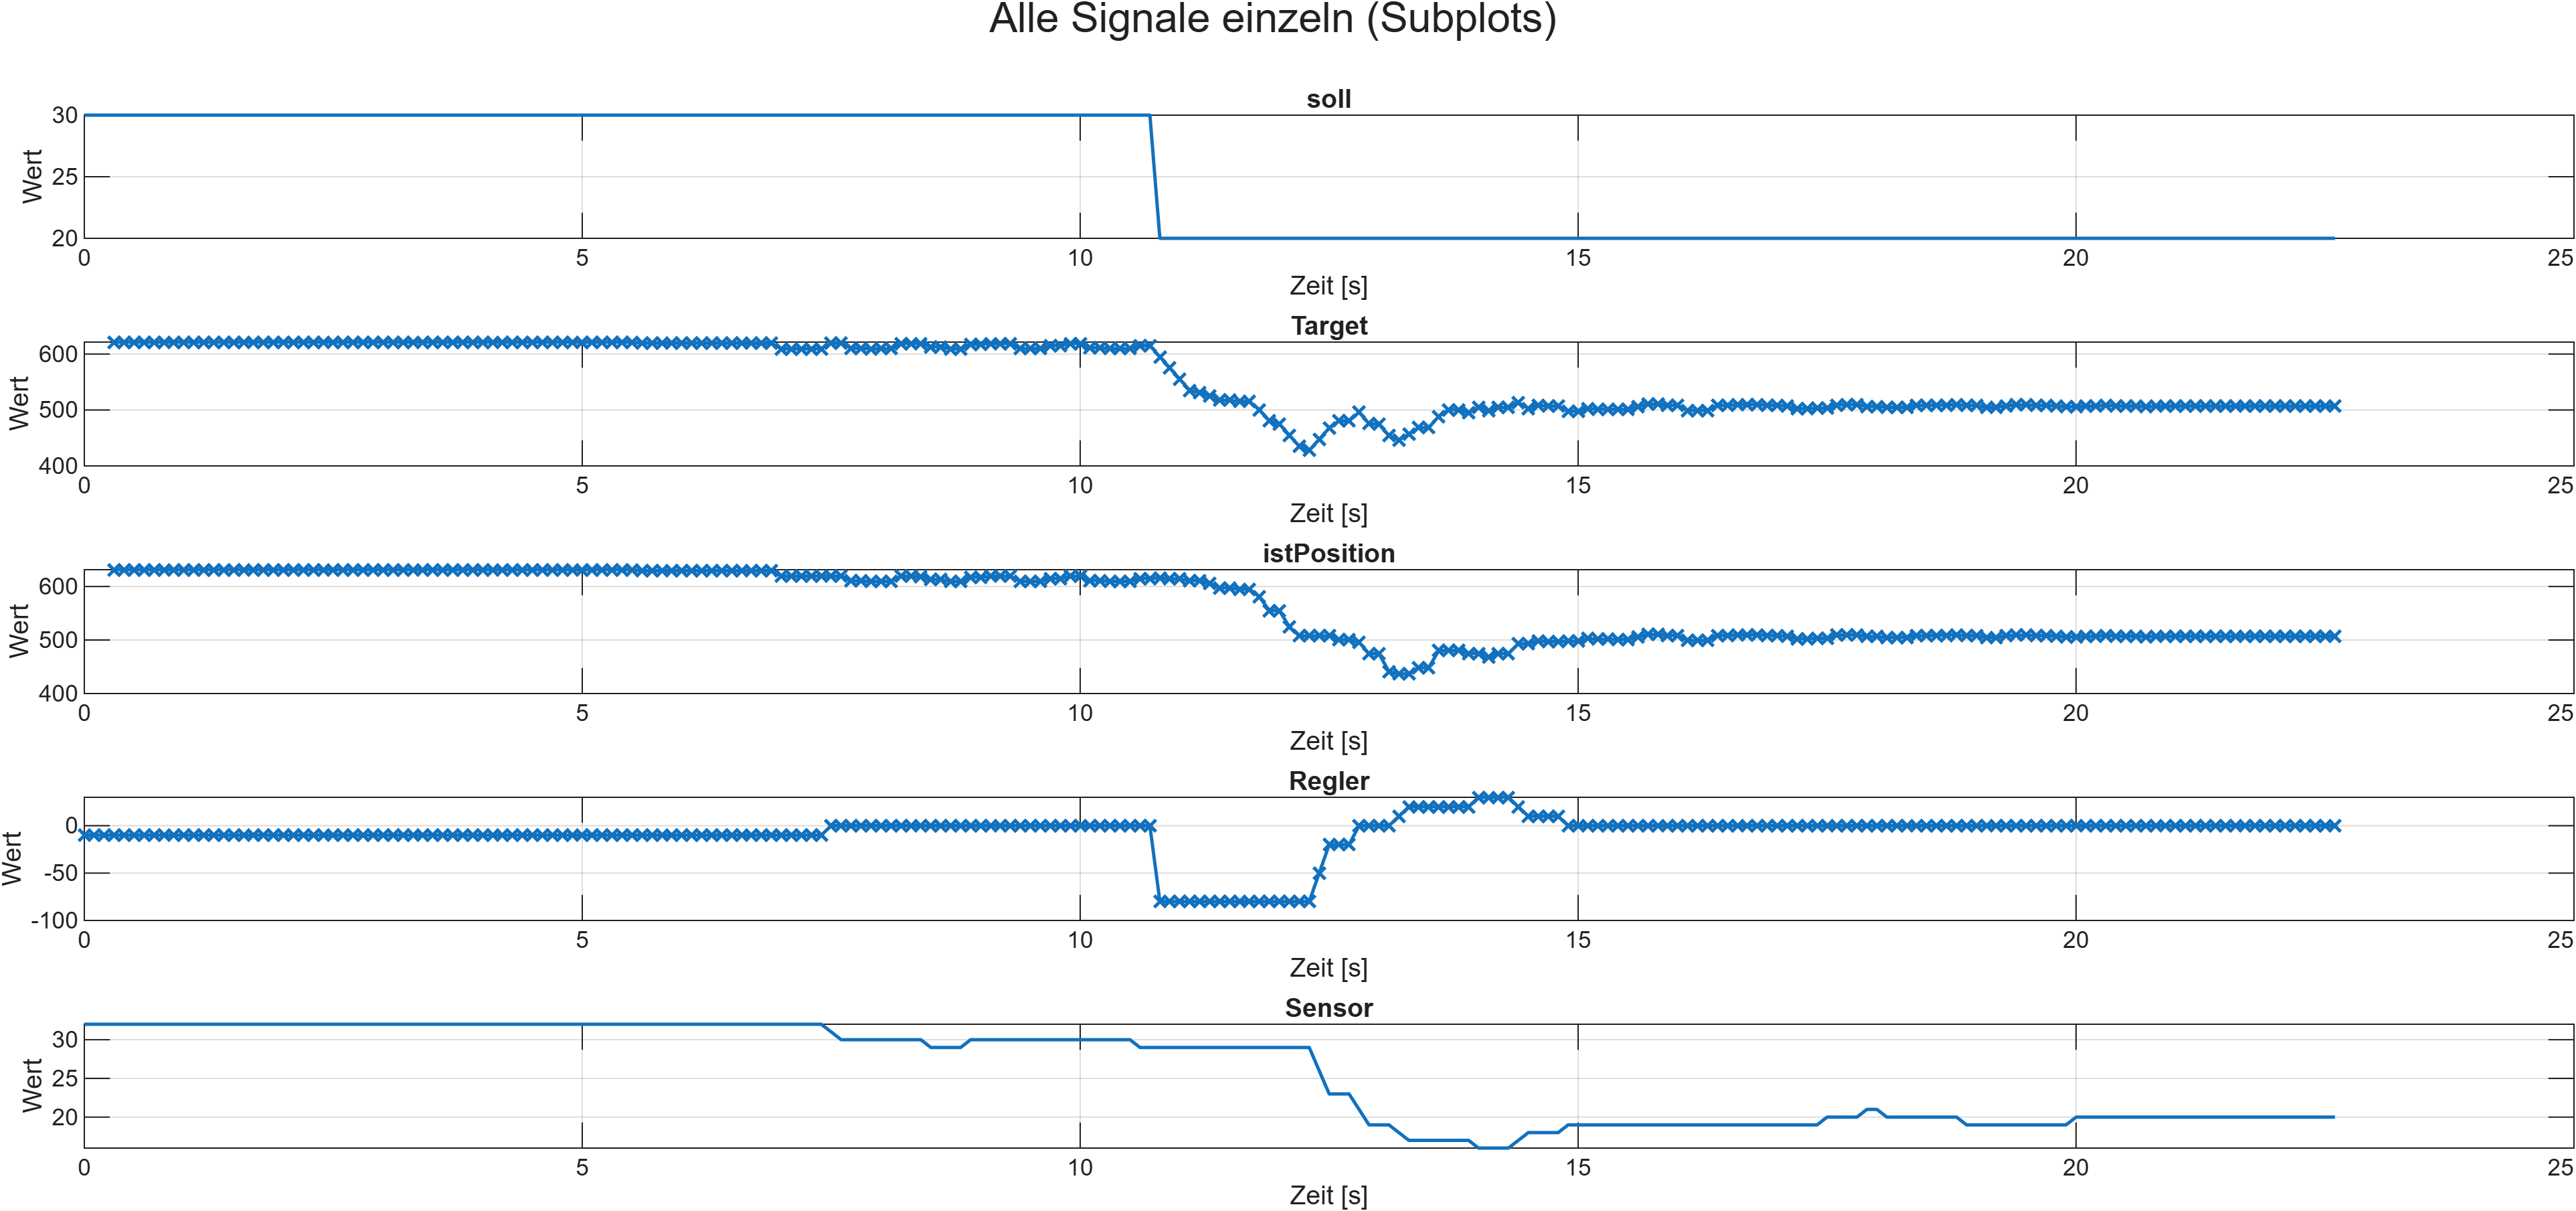
\includegraphics[width=0.9\linewidth]{images/realsensor_signale_einzeln.png}
    \caption{Sprungversuch am realen Ultraschallsensor: Einzeldarstellung
    aller fünf Signale.}
    \label{fig:realsensor_einzeln}
\end{figure}

Vor dem Sprung befinden sich \texttt{Target} und \texttt{istPosition}
praktisch deckungsgleich bei \SI{615.0}{\milli\meter}. Nach dem Sprung
überschwingt \texttt{Target} auf ein Minimum von \SI{427.7}{\milli\meter}
bei $t=\SI{12.3}{\second}$, \texttt{istPosition} folgt mit einer leichten
Verzögerung auf ein Minimum von \SI{436.6}{\milli\meter} bei
$t=\SI{13.2}{\second}$; beide pendeln sich anschließend auf den
gemeinsamen Endwert von \SI{506.9}{\milli\meter} ein. Bezogen auf die
Sprunghöhe von \SI{108.1}{\milli\meter} entspricht dies einem deutlichen
Überschwingen von rund \SI{70}{\percent}; dies ist ein Hinweis auf ein eher
schwach gedämpftes Übertragungsverhalten der aktuellen Reglerauslegung,
das im Abschnitt zur Reglerparametrierung weiter untersucht werden sollte.

Anhand des Zeitversatzes zwischen \texttt{Target} und \texttt{istPosition}
(Nulldurchgang jeweils beim Mittelwert zwischen Ausgangs- und Endwert)
ergibt sich eine erste grobe Schätzung der Gesamt-Totzeit des Systems von
rund \SI{0.8}{\second}; eine genauere Bestimmung erfolgt im nachfolgenden
Abschnitt zur Totzeit.

Der Reglerausgang (\texttt{Regler}) liegt vor dem Sprung bei $\approx 0$
und springt exakt mit dem Sollwertsprung auf seinen unteren Grenzwert von
$-80$, an dem er für \SI{1.5}{\second} ($t=\SI{10.8}{\second}$ bis
$\SI{12.3}{\second}$) verharrt, bevor er durch Null läuft, kurzzeitig
positiv auf bis zu $+30$ überschwingt ($t\approx\SI{14.0}{\second}$) und
sich anschließend wieder bei $\approx 0$ einpendelt. Die über 16
aufeinanderfolgende Samples exakt konstante Auslenkung deutet auf eine
reale Begrenzung (Sättigung) des Stellsignals hin, die während der starken
initialen Korrekturbewegung aktiv wird (namensgebend für den Ordner
\texttt{Real Sensor Test with Saturation} dieser Messung).
% TODO: Zusammenhang zwischen dieser Stellgrößen-Sättigung und einer
% möglichen Totzone des Reglers noch zu klären (Rücksprache im Team
% ausstehend).

Die Sensor-Messung selbst pendelt sich nach dem Sprung mit einer
Restabweichung von nur \SI{-0.1}{\centi\meter} praktisch exakt auf den
neuen Sollwert von \SI{20}{\centi\meter} ein.

%% TODO: noch offen -- Inhalt folgt, sobald die entsprechenden
%% Projektarbeiten (Anforderungen 1, 2, 4) durchgeführt wurden.
